

\def\mystudentname{Oliver Racey}

\def\mysupervisor{Idris Ibrahim} 

\def\mytitle{Intelligent Image Analysis of Electrocardiograms}

\def\mydegree{BSc Computer Science }

\def\mydepartment{School of Mathematics and Computer Science}

\def\myuniversityname{Heriot-Watt University}

%% ---------------------------------------------


\documentclass[oneside,a4paper,11pt]{book}

%%-----------------         

%\usepackage{mathptmx}
%\usepackage{anyfontsize}
%\usepackage{t1enc}
\usepackage{amsmath}
\usepackage[document]{ragged2e}

%%-----------------         


% Adjust margins
\addtolength{\oddsidemargin}{-0.6in}
\addtolength{\evensidemargin}{-0.6in}
\addtolength{\textwidth}{1.2in}
%
\addtolength{\topmargin}{-.15in}
\addtolength{\textheight}{0.30in}

%%%-----------------

\usepackage{graphicx}
\usepackage{float}
\usepackage{booktabs}
\graphicspath{{./images/}} % Specifies the directory where pictures are stored

%% ----

\renewcommand{\thefigure}{\arabic{chapter}.\arabic{figure}}
%\renewcommand{\thefigure}{A\arabic{section}.\arabic{figure}}
%\counterwithout{section}{chapter}
%\counterwithin{chapter}{part}

%% ----

\usepackage[absolute,overlay]{textpos}

\usepackage{lastpage}

%% -------------------------------------------------------
\usepackage{pgfgantt} % to create gantt char
\usetikzlibrary{positioning,arrows.meta,fit} % to create diagrams in latex
\usepackage{longtable}
\usepackage{hyperref}
\usepackage{subcaption} % figures side by side
\usepackage[table]{xcolor}
\newcommand{\High}{\cellcolor{red!90}High}
\newcommand{\Med}{\cellcolor{yellow!90}Medium}
\newcommand{\Low}{\cellcolor{green!90}Low}

\hypersetup{
	colorlinks = true, 
	linkcolor = black,
	anchorcolor = red,
	citecolor = blue, 
	filecolor = black, 
	%urlcolor = red,
}

%%%-----------------

\usepackage{makeidx}
\makeindex

\setlength{\parindent}{0pt} % remove indent

\renewcommand{\contentsname}{Table of Contents}

\usepackage[
    backend=biber,
    style=ieee,
    sorting=none
]{biblatex}
% ---- Fit figures and tables closer to the text ----
\renewcommand{\topfraction}{0.9}        % floats may fill 90% of the top of a page
\renewcommand{\bottomfraction}{0.8}     % ... and 80% of the bottom
\renewcommand{\textfraction}{0.07}      % a page needs only 7% text
\renewcommand{\floatpagefraction}{0.8}  % float-only pages must be 80% full
\setcounter{topnumber}{3}
\setcounter{bottomnumber}{3}
\setcounter{totalnumber}{5}
\setlength{\textfloatsep}{10pt plus 2pt minus 4pt}  % gap between floats and text
\setlength{\floatsep}{8pt plus 2pt minus 2pt}       % gap between two floats
\setlength{\intextsep}{8pt plus 2pt minus 2pt}      % gap around [h] / [H] floats
\setlength{\abovecaptionskip}{4pt}
\setlength{\belowcaptionskip}{2pt}

% ---- Compact chapter headings (book class default leaves ~1/4 page blank) ----
\makeatletter
\renewcommand{\@makechapterhead}[1]{%
  \vspace*{0pt}%
  {\parindent \z@ \raggedright \normalfont
    \ifnum \c@secnumdepth >\m@ne
      \if@mainmatter
        {\Large\bfseries \@chapapp\space \thechapter}\par\nobreak
        \vskip 6\p@
      \fi
    \fi
    {\LARGE \bfseries #1}\par\nobreak
    \vskip 18\p@}}
\renewcommand{\@makeschapterhead}[1]{%
  \vspace*{0pt}%
  {\parindent \z@ \raggedright \normalfont
    {\LARGE \bfseries #1}\par\nobreak
    \vskip 18\p@}}
\makeatother

% ---- Slightly tighter spacing around section headings ----
\makeatletter
\renewcommand{\section}{\@startsection{section}{1}{\z@}%
  {-2.4ex \@plus -0.6ex \@minus -.2ex}{1.3ex \@plus .2ex}{\normalfont\Large\bfseries}}
\renewcommand{\subsection}{\@startsection{subsection}{2}{\z@}%
  {-2ex \@plus -0.5ex \@minus -.2ex}{1ex \@plus .2ex}{\normalfont\large\bfseries}}
\makeatother
\addbibresource{image_processing_bibliography.bib}

\begin{document}
	\frontmatter
	
% titlepage

\begin{titlepage}
\begin{textblock}{4}(1.5,14.5)
	\small 
	Number Pages:  \pageref{LastPage}\\
	Word Count: x
\end{textblock}
	\begin{center}
		\vspace*{1cm}
		
		{\fontsize{25pt}{30pt}\selectfont
		 \textbf{\mytitle} \par}
	
		
		\vspace{1.5cm}
		
		{\LARGE
		\textbf{\mystudentname}
	    }
	
		\vspace{3.0cm}
		{\fontsize{12pt}{12pt}\selectfont \mydepartment}
		
		\vfill
		
		A thesis presented for the degree of\\
		\mydegree
		
		\vspace{0.8cm}
		
		
\includegraphics[width=0.3\textwidth]{HWUlogo.jpg}
		
		\vspace{2.5cm}
		
		% \mydepartment\\
		\myuniversityname\\
		\today
		
	\end{center}
\end{titlepage}



% copyright
\newpage
\addcontentsline{toc}{chapter}{Declaration of Authorship}
{\fontsize{18pt}{18}\selectfont\textbf{Declaration of Authorship}}
\vspace{1.5cm}

I, \mystudentname, declare that this thesis titled, `\mytitle' and thework presented in it is my own. I confirm that this work submitted for assessment is myown and is expressed in my own words. Any uses made within it of the works of otherauthors in any form (e.g., ideas, equations, figures, text, tables, programs) are properly acknowledged at any point of their use. A list of the references employed is included.
\vspace{1.5cm}

Signed:  

\vspace{1.5cm}

Dated: 



% dedication

% abstract
\newpage
\addcontentsline{toc}{chapter}{Abstract}
\thispagestyle{plain}
\begin{center}
	{
	\Large
	\textbf{\mytitle}
	
	\vspace{0.4cm}
	\textbf{\mystudentname}
	
	\vspace{0.9cm}
	\textbf{Abstract}
	\vspace{0.5cm}
    }

    \begin{justify}
    Electrocardiograms are often the most common form of tests for the heart. Many of these ECGs exist only as prints or photos. This means that any analysis has to be undertaken in person, so transferring this information into a digital world has issues. Digital classifiers that do work on ECG images have mostly been tested on synthesised images, whilst rarely reporting if the classifer can be verified in its results. Therefore, this project will develop a convolutional neural network (known as a CNN), as well as an application, that flags cardiac abnormalities in ECG images. It also reports a confidence score, and explains any predictions it has made using heatmaps. A multi-faced GUI, one for users, whilst another for clinicans, are created to present this information to multiple types of users. The model will be trained on images rendered from PTB-XL, and then tested on real scanned and photographed ECGs, across 5 diagnostic superclasses and four ryhthm classes. The performance will be measured per class, with metrics suited to imbalanced data. Confidence will be calibrated with temperature sclaing, and the Graphical User Interface (GUI) will be evaluated in a user study, where the ethics approval has been granted. Prototypes showing image rendering, preprocessing, and interface wireframes, show that this plan is feasible. The project is expected to show how far the performance and calibration hold when going from rendered to real images, and whether non-experienced users can interpret the results. 
    \end{justify}
	
\end{center}


% Contents and lists
% Each list starts on a fresh page. LaTeX writes the entries to auxiliary
% files on one run and displays them on the next run.
\cleardoublepage
\pagestyle{plain}

\phantomsection
\addcontentsline{toc}{chapter}{Table of Contents}
\tableofcontents

\cleardoublepage
\phantomsection
\addcontentsline{toc}{chapter}{List of Figures}
\listoffigures

\cleardoublepage
\phantomsection
\addcontentsline{toc}{chapter}{List of Tables}
\listoftables

\cleardoublepage

% abreviations
\addcontentsline{toc}{chapter}{Abbreviations}

\clearpage
\newpage

{\Huge \textbf{Abbreviations}}
\vspace{1.0cm}

\begin{table*}[!h]
  \centering
  \begin{tabular}{ll}

\textbf{AFIB} & \textbf{A}trial \textbf{Fib}rillation \\
\textbf{AFLT} & \textbf{A}trial \textbf{F}lutter \\
\textbf{AUROC} & \textbf{A}rea \textbf{U}nder the \textbf{R}eceiver \textbf{O}perating \textbf{C}haracteristic Curve \\
\textbf{CD} & \textbf{C}onduction \textbf{D}isturbance \\
\textbf{CLAHE} & \textbf{C}ontrast \textbf{L}imited \textbf{A}daptive \textbf{H}istogram \textbf{E}qualization \\
\textbf{CNN} & \textbf{C}onvolutional \textbf{N}eural \textbf{N}etwork \\
\textbf{ECE} & \textbf{E}xpected \textbf{C}alibration \textbf{E}rror \\
\textbf{ECG} & \textbf{E}lectro \textbf{c}ardio\textbf{g}ram \\
\textbf{FR} & \textbf{F}unctional \textbf{R}equirements\\
\textbf{GPU} & \textbf{G}raphical \textbf{P}rocessing \textbf{U}nit \\
\textbf{Grad-CAM} & \textbf{G}radient-weighted \textbf{C}lass \textbf{A}ctivation \textbf{M}apping \\
\textbf{GUI} & \textbf{G}raphical \textbf{U}ser \textbf{I}nterface \\
\textbf{HE} & \textbf{H}istogram \textbf{E}qualization\\
\textbf{HR} & \textbf{H}eart \textbf{R}ate\\
\textbf{HYP} & \textbf{Hyp}ertrophy \\
\textbf{MCC} & \textbf{M}atthews \textbf{C}orrelation \textbf{C}oefficient \\
\textbf{MI} & \textbf{M}yocardial \textbf{I}nfarction \\
\textbf{MoSCoW} & \textbf{Mu}st, \textbf{S}hould, \textbf{Co}uld, \textbf{W}on't \\
\textbf{NFR} & \textbf{N}on-\textbf{F}unctional \textbf{R}equirements\\
\textbf{NORM} & \textbf{Norm}al ECG \\
\textbf{Obj} & \textbf{Obj}ective \\
\textbf{QRS / QT / PR} & ECG waveform complex and intervals \\
\textbf{RR} & Interval between successive R peaks \\
\textbf{RTM} & \textbf{R}equirements \textbf{T}raceability \textbf{M}atrix \\
\textbf{SBRAD} & \textbf{S}inus \textbf{Brad}ycardia \\
\textbf{SD} & \textbf{S}tandard \textbf{D}eviation \\
\textbf{SNR} & \textbf{S}ignal-to-\textbf{N}oise \textbf{R}atio \\
\textbf{SQ} & \textbf{S}ub \textbf{Q}uestion \\ 
\textbf{STACH} & \textbf{S}inus \textbf{Tach}ycardia \\
\textbf{STTC} & \textbf{ST/T} \textbf{C}hange \\
\textbf{SUS} & \textbf{S}ystem \textbf{U}sability \textbf{S}cale \\
\textbf{TC} & \textbf{T}est \textbf{C}ase \\
  \end{tabular}
\end{table*}

\newpage

	\mainmatter
	\chapter{Introduction}
\label{ch:intro}

\section{Context and Motivation}

The electrocardiogram (ECG) is one of the most common heart tests, but interpretation is difficult: clinicians can disagree about the same trace \cite{dhutia_interrater_2017}, and readings need to be reviewed by experienced readers \cite{schlapfer_computer-interpreted_2017}. Many ECGs are stored as prints or photographs, which automated analysis built for digital signals cannot use \cite{shivashankara_ecg-image-kit_2024}.

\section{Problem Statement}
\label{sec:problem}

Deep learning models classify ECGs well when given raw signal data
\cite{hannun_cardiologist_2019,ribeiro_automatic_2020}. Work on images is newer, and
Chapter~\ref{ch:lit} shows that it is limited in four ways:
\begin{enumerate}\setlength{\itemsep}{0pt}\setlength{\parskip}{0pt}
  \item Image-based classifiers have mostly been tested on synthesised images, or on a limited set of real images.
  \item Image-based studies rarely report whether the model's confidence scores are calibrated.
  \item Explanations of the predictions are rarely evaluated.
  \item There is little evidence on how results should be presented to different kinds of users.
\end{enumerate}
A system that flags possible abnormalities from real ECG images, states its confidence and shows what each prediction was based on would address these gaps. It must also cope with rendering shortcuts, a grid that is the only record of scale, and imbalanced classes.

\section{Aim and Objectives}

\textbf{Aim.} To build and evaluate a convolutional neural network (CNN) application that
flags possible abnormalities from ECG images, reports its calibrated confidence, and explains its predictions to different users. The system is a supportive review and is not a diagnostic tool to replace health professionals' advice.

\begin{enumerate}\setlength{\itemsep}{0pt}\setlength{\parskip}{0pt}
  \item \textbf{O1:} Render a labelled training set from PTB-XL with ECG-Image-Kit, and assemble a real test set from the ECG-Image-Database.
  \item \textbf{O2:} Develop a preprocessing and waveform-detection pipeline that detects the trace and the beats.
  \item \textbf{O3:} Train a multi-label CNN and evaluate it with imbalance-aware metrics on patient-wise splits.
  \item \textbf{O4:} Measure the drop in performance from rendered to real images.
  \item \textbf{O5:} Calibrate confidence with temperature scaling; report calibration error per class.
  \item \textbf{O6:} Explain predictions with Grad-CAM in a GUI for different users, and run a user study.
\end{enumerate}
	\chapter{Literature Review}
\label{ch:lit}
\section{Introduction}

This chapter moves from general image processing to ECG-specific methods, classifiers and existing systems, and argues that image-based ECG classifiers have mostly been tested on synthesised images, with little attention to their confidence and explanations. Abbreviations and technical terms are defined in the Glossary.

\section{Digital Image Processing}
\label{sec:image-processing}

A digital image is a two-dimensional function $f(x,y)$ whose value at each pixel is the intensity at that point \cite{gonzalez_digital_2018}. The intensity is the product of the illumination $i$ and the reflectance $r$ of the surface, $f(x,y) = i(x,y)\,r(x,y)$ \cite{stockham_image_1972}, so one object, or one ECG trace, can look different under different lighting. Images are digitised by sampling into pixels and quantising each value to a finite number of levels, which discards detail irreversibly \cite{gonzalez_digital_2018}.

Processing then enhances the image for a task, removes noise, and segments it into meaningful regions. Table~\ref{tab:techniques} summarises the main techniques and their trade-offs. No single method suits every image, as removing noise can also distort real detail, so the choice depends on the degradation and the task \cite{qi_comprehensive_2022}.

\begin{table}[!htbp]
  \centering
  \footnotesize
  \renewcommand{\arraystretch}{1.15}
  \caption{Image processing techniques relevant to ECG images, and their trade-offs.}
  \label{tab:techniques}
  \begin{tabular}{@{}p{0.27\linewidth} p{0.30\linewidth} p{0.37\linewidth}@{}}
    \toprule
    \textbf{Technique} & \textbf{Use} & \textbf{Trade-off} \\
    \midrule
    Histogram equalisation (HE) & Spreads intensities to raise contrast & Handles local detail poorly \\
    CLAHE \cite{pizer_adaptive_1987,zuiderveld_contrast_1994} & Local contrast, uneven lighting & Clip limit must be tuned; can raise noise \\
    Gaussian filter \cite{gonzalez_digital_2018} & Reduces random noise & Blurs edges and thin peaks \\
    Median filter & Removes salt-and-pepper noise & Can flatten narrow peaks \\
    Bilateral filter \cite{tomasi_bilateral_1998,verma_ali_2013} & Smooths flat regions, keeps edges & Slower; needs tuning \\
    Non-local means \cite{buades_non-local_2005} & Noise removal using similar patches & Computationally expensive \\
    Notch filter (Fourier domain) \cite{gonzalez_digital_2018} & Removes regular patterns such as the grid & Struggles with faded or monochrome prints \\
    Homomorphic filter \cite{stockham_image_1972} & Suppresses illumination $i$, boosts reflectance $r$ & Can amplify noise \\
    Wavelet transform \cite{lepcha_deep_2023} & Multi-scale noise removal & Choice of scale and threshold \\
    Thresholding (Otsu) \cite{otsu_threshold_1979} & Separates trace from background & Fails under uneven lighting \\
    Edge detection \cite{canny_computational_1986} and morphology & Finds and cleans up boundaries & Sensitive to noise \\
    \bottomrule
  \end{tabular}
\end{table}

\section{Medical Image Processing}
\label{sec:medical-imaging}

Medical images must preserve diagnostic detail, which noise can obscure \cite{prasad_systematic_2023}, and their quality is best defined by how well an observer performs a task, not by appearance \cite{barrett_foundations_2004}. CNNs, which learn filters from labelled examples \cite{lecun_gradient_1998}, are now used across medical imaging \cite{litjens_survey_2017}, but labelled data is expensive, performance may not carry over to new hospitals, as pneumonia detectors performed differently across three hospital systems \cite{zech_variable_2018}, and models may rely on shortcuts that correlate with the label \cite{geirhos_shortcut_2020}. Systems should therefore explain their output \cite{selvaraju_gradcam_2017} and report calibrated confidence \cite{guo_calibration_2017}. In this project, preprocessing will be judged by its effect on classification, and the rendered-to-real gap is treated as a generalisation problem.

\section{ECG Fundamentals}
\label{sec:ecg-fundamentals}

The ECG is an electrical tracing of the heart recorded from the body surface \cite{sattar_electrocardiogram_2023}. Each heartbeat produces a P wave (atrial activation), a QRS complex (ventricular activation) and a T wave (recovery), and the intervals between them carry diagnostic information (Figure~\ref{fig:ecg-beat}): the PR interval reflects the delay from atria to ventricles, the QRS duration how quickly the ventricles activate, and the QT interval spans ventricular activation and recovery. A standard resting ECG records twelve leads, each viewing the heart from a different direction, printed as short pieces on a $3\times4$ layout \cite{ashley_conquering_2004} (Figure~\ref{fig:ecg-grid}). On the grid, distance and deflection convert to time and voltage by $t = x/v$ and $V = y/g$, with standard paper speed $v=25$\,mm/s and gain $g=10$\,mm/mV \cite{sattar_electrocardiogram_2023}; the heart rate follows from the RR interval as $\mathrm{HR} = 60/\mathrm{RR}$. Timing and amplitude can only be read from an image if the grid calibration is known, so skewing, cropping or photographing the page distorts them.

\begin{figure}[!htbp]
  \centering
  \begin{minipage}[b]{0.42\linewidth}
    \centering
    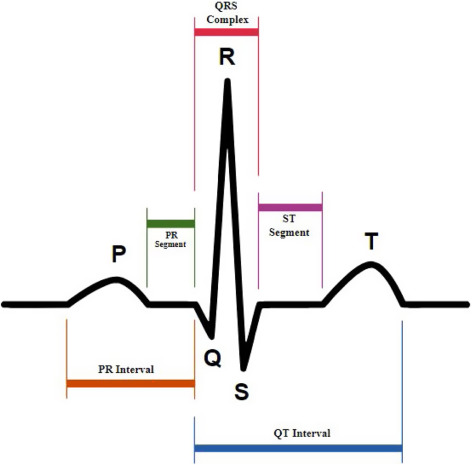
\includegraphics[width=0.7\linewidth,height=0.18\textheight,keepaspectratio]{images/LabelledHeartbeat.jpg}
    \caption[A single PQRST wave]{A single heartbeat with its main waves and intervals. Generated by the author from \cite{Mazomenos_ECG_2012}.}
    \label{fig:ecg-beat}
  \end{minipage}\hfill
  \begin{minipage}[b]{0.52\linewidth}
    \centering
    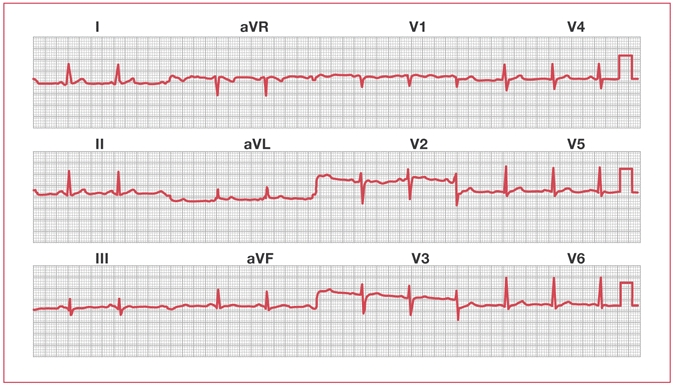
\includegraphics[width=0.7\linewidth,height=0.18\textheight,keepaspectratio]{images/ECGGrid.jpg}
    \caption[An ECG paper trace]{A twelve-lead ECG printed as a $3\times4$ grid of leads \cite{ashley_conquering_2004}.}
    \label{fig:ecg-grid}
  \end{minipage}
\end{figure}

Arrhythmias change the rate or rhythm \cite{nhs_heart_2018}: atrial fibrillation has irregular beats without clear P waves \cite{van_gelder_2024_2024}, and atrial flutter a saw-tooth pattern \cite{cosio_atrial_2017}. Bundle branch blocks widen the QRS complex \cite{scherbak_left_2024}, MI alters the ST segment and T wave, and hypertrophy changes amplitudes \cite{channer_myocardial_2002}. Some classes thus depend on shape and others on timing, which in an image depends on the grid scale. PTB-XL labels 21,800 twelve-lead ECG signals from about 19,000 patients with five diagnostic superclasses (normal, MI, ST/T change, conduction disturbance, hypertrophy) and rhythm statements, allowing several labels per record \cite{wagner_ptbxl_2020}.

\section{ECG Imaging and Digitisation}
\label{sec:ecg-imaging}

Printed or photographed ECGs cannot be used by signal-based software \cite{shivashankara_ecg-image-kit_2024}, and they vary in lighting, artefacts and camera angle \cite{reyna_ecg-image-database_2024}; \textcite{gliner_domain_2023} needed domain adaptation to move a model from scans to phone images, and image resolution limits how accurately timing can be measured. There are two approaches.

\subsection{ECG Digitisation Approach}
\label{sec:digitisation}

Digitisation reconstructs the signal from the image, by locating the grid, separating the leads and tracing each waveform, so that signal-based methods can be applied. It gives measurable intervals, but an error at any step carries into the reconstructed signal. The PhysioNet Challenge 2024 evaluated digitisation by the SNR of the recovered signal \cite{physionet_challenge_2024}.

\subsection{Direct Classification Approach}
\label{sec:direct-classification}

Direct classification avoids reconstruction, but the model must learn timing from pixels, so its results depend on how the images were produced. Two data sources support it: ECG-Image-Kit generates synthesised images with artefacts from real signals \cite{shivashankara_ecg-image-kit_2024}, and the ECG-Image-Database provides about 36,000 images of PTB-XL and Emory Healthcare records that were printed, degraded, and scanned or photographed \cite{reyna_ecg-image-database_2024}; a smaller set of real images with varied degradation is also available \cite{khan_ecg_2021}. This project will classify images directly, training on images rendered from PTB-XL and testing on real images, so that the effect of real imaging conditions can be measured.

\section{Pre-processing and Noise Removal}
\label{sec:preprocessing}

Preprocessing applies the methods of Table~\ref{tab:techniques} to faults from printing and capture, with ECG-specific risks. The grid can confuse a classifier but is the only record of scale, so it must be measured before removal; the trace is only a few pixels wide, so smoothing can erase P waves and QRS peaks; rotation correction cannot fully undo the perspective of a photograph; and a CNN trained on varied images may not need preprocessing at all. Preprocessing will therefore be judged by its effect on classification.

\section{Feature Extraction}
\label{sec:features}

Classical ECG analysis measured hand-designed features, such as interval lengths and wave amplitudes, and passed them to a classifier \cite{de_chazal_automatic_2004}. These have clear clinical meaning, and RR regularity separates regular from irregular rhythms, but they depend on every earlier step succeeding. A CNN instead learns features from the pixels \cite{lecun_deep_2015}, which avoids this dependency but is harder to explain and needs more data. Figure~\ref{fig:feature-extraction} compares the two routes. This project will combine them: learned features suit the shape-based superclasses, and measured timing features (Section~\ref{sec:waveform}) support the rhythm classes.

\begin{figure}[!htbp]
  \centering
  \makebox[\linewidth][c]{%
  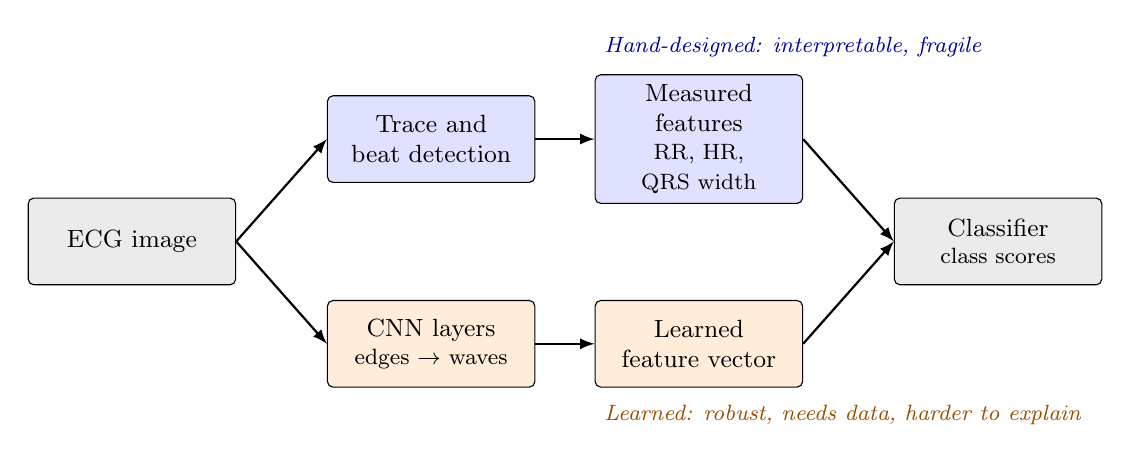
\begin{tikzpicture}[
      font=\small,
      box/.style={draw, rounded corners=2pt, align=center, minimum height=11mm,
                  text width=24mm, fill=#1},
      box/.default=white,
      arr/.style={-latex, thick}
    ]
    \node[box=black!8] (img) at (0,0) {ECG image};
    \node[box=blue!12] (det) at (38mm,13mm) {Trace and beat detection};
    \node[box=blue!12] (meas) at (72mm,13mm) {Measured features\\[-1pt]\footnotesize RR, HR, QRS width};
    \node[box=orange!15] (conv) at (38mm,-13mm) {CNN layers\\[-1pt]\footnotesize edges $\rightarrow$ waves};
    \node[box=orange!15] (learn) at (72mm,-13mm) {Learned feature vector};
    \node[box=black!8] (clf) at (110mm,0) {Classifier\\[-1pt]\footnotesize class scores};

    \draw[arr] (img.east) -- (det.west);
    \draw[arr] (det) -- (meas);
    \draw[arr] (meas.east) -- (clf.west);
    \draw[arr] (img.east) -- (conv.west);
    \draw[arr] (conv) -- (learn);
    \draw[arr] (learn.east) -- (clf.west);

    \node[anchor=south west, font=\footnotesize\itshape, text=blue!60!black]
      at ([yshift=1mm]meas.north west) {Hand-designed: interpretable, fragile};
    \node[anchor=north west, font=\footnotesize\itshape, text=orange!60!black]
      at ([yshift=-1mm]learn.south west) {Learned: robust, needs data, harder to explain};
  \end{tikzpicture}%
  }
  \caption{Hand-designed and learned feature extraction from an ECG image. This project
    will pass timing features from detected beats to the classifier alongside the features the CNN learns.}
  \label{fig:feature-extraction}
\end{figure}

\section{Waveform Detection}
\label{sec:waveform}

In signals, waveform detection usually locates the QRS complex; the Pan--Tompkins algorithm band-pass filters, differentiates and squares the signal, then applies adaptive thresholds \cite{pan_real-time_1985}. In images, the trace must first be found: published pipelines binarise the image, remove the grid and text, locate each lead with a Hough transform, and reduce each column of the trace to one value before converting it to time and voltage \cite{wu_automated_2022}. Detection can be accurate, with correlations of 0.94 \cite{randazzo_development_2022} and about 0.99 on standard layouts \cite{wu_automated_2022} against reference signals, but it is fragile: correlation fell to about 0.96 on printed and rescanned ECGs \cite{wu_automated_2022}, and a missed peak corrupts every timing feature that follows. This project will therefore evaluate detection on real images, not only rendered ones.

\section{ECG Classification Algorithms}
\label{sec:ml-ecg}

Deep learning has largely replaced feature-based ECG classification. On signals, networks reached cardiologist-level rhythm classification (F1 0.837 against 0.780 for cardiologists) \cite{hannun_cardiologist_2019}, outperformed residents on 12-lead abnormalities \cite{ribeiro_automatic_2020}, and convolutional architectures performed best on PTB-XL \cite{strodthoff_deep_2021}. Image-based work is newer and relies on transfer learning from networks such as ResNet pretrained on natural images \cite{he_deep_2016,yosinski_transfer_2014}; the main image-based systems are compared in Section~\ref{sec:existing-systems}, and the key signal and image studies are summarised in Table~\ref{tab:ecg-studies} (Appendix~\ref{app:lit}). Signal results do not transfer directly to images, which carry their scale only through the grid. Labels also limit all studies: PTB-XL's come from at most two cardiologists \cite{wagner_ptbxl_2020}, who can disagree \cite{dhutia_interrater_2017}, and differing datasets and metrics mean headline numbers cannot be ranked directly.

\section{ECG Dataset Evaluation}
\label{sec:ml-eval}

ECG datasets are imbalanced, so accuracy can be high even when rare conditions are missed; sensitivity, specificity and MCC give a truer picture \cite{chicco_advantages_2020}, and data should be split by patient using PTB-XL's suggested folds \cite{wagner_ptbxl_2020}. Overconfident networks can be calibrated by temperature scaling \cite{guo_calibration_2017}: each class score $z_k$ is divided by a temperature $T$ fitted on validation data, $\hat{p}_k = \sigma(z_k/T)$, leaving AUROC unchanged, and calibration is measured by the ECE. Applying this to independent sigmoid outputs is an adaptation, and calibration deteriorates under data shift \cite{ovadia_trust_2019}, so whether it survives the move to real images must be measured. Grad-CAM heatmaps show which regions influenced a prediction \cite{selvaraju_gradcam_2017}, but some saliency maps barely change when a model's weights are randomised \cite{adebayo_sanity_2018}, so heatmaps must be checked against known cases.

\section{Existing Systems and Limitations}
\label{sec:existing-systems}

Most ECGs are analysed by the recording machine's software, but its accuracy is limited, so over-reading by an experienced reader is needed, and it cannot analyse printouts \cite{schlapfer_computer-interpreted_2017}. Table~\ref{tab:existing-systems} compares this with the main deep-learning systems.

\begin{table}[H]
  \centering
  \footnotesize
  \renewcommand{\arraystretch}{1.1}
  \caption{Comparison of existing ECG analysis systems and the planned system.}
  \label{tab:existing-systems}
  \begin{tabular}{@{}p{0.17\linewidth} p{0.17\linewidth} p{0.27\linewidth} p{0.31\linewidth}@{}}
    \toprule
    \textbf{System} & \textbf{Input} & \textbf{Key features} & \textbf{Limitations} \\
    \midrule
    ECG machine software \cite{schlapfer_computer-interpreted_2017} &
      Digital signal at recording &
      Immediate automated report &
      Limited accuracy, needs over-reading; cannot analyse printouts or images \\
    \textcite{sangha_automated_2022} &
      Images generated from signals &
      CNN tested on held-out, external and printed ECGs (AUROC 0.98) &
      Trained on generated images; reports discrimination only, not calibration \\
    \textcite{gliner_domain_2023} &
      Scans; phone-captured frames &
      Domain adaptation from scans to phone images (AUROC 0.91) &
      Phone images made by filming printed pages; six unseen formats tested \\
    \textcite{wang_pipeline_2025} &
      Synthetic and external scanned images &
      Challenge-winning ConvNeXt pipeline (AUROC about 0.97) &
      Evaluated on synthetic PTB-XL images, with possible leakage \\
    \textcite{chen_quantifying_2022} &
      Digital signals &
      Uncertainty estimates for atrial fibrillation; improved calibration &
      Signals only, one condition \\
    \midrule
    This project (planned) &
      Rendered images for training; real images for testing &
      Multi-label CNN with timing features; calibrated confidence; Grad-CAM; views for different users; user study &
      Labels from at most two annotators; real test set limited to the ECG-Image-Database \\
    \bottomrule
  \end{tabular}
\end{table}

Four gaps remain. First, image-based classification has mostly been tested on synthetic or limited real images (Table~\ref{tab:existing-systems}). Second, calibration has been studied for signals \cite{chen_quantifying_2022}, but image-based studies report only discrimination. Third, explanations are seldom assessed: 43\% of explainable-AI studies in cardiology did not evaluate them, and only 11\% involved clinicians \cite{salih_review_2024}. Fourth, presentation depends on the user: clinicians preferred visualisations of what the algorithm analysed \cite{hughes-noehrer_contrasting_2024}, and explanations raised novices' trust more than experts' \cite{cabitza_painting_2023}. Datasets also reflect limited settings: PTB-XL was collected between 1989 and 1996 with devices from one manufacturer \cite{wagner_ptbxl_2020}, so models may not generalise.

\section{Summary}
\label{sec:lit-summary}

Reading an ECG from an image combines an image problem, recovering a measurable trace from a degraded picture, with a clinical problem, deciding what the trace shows. Signal-based deep learning is mature, but image-based work has relied on synthetic data and paid little attention to whether its confidence can be trusted or its explanations understood. This project will address the four gaps in turn: a preprocessing and detection pipeline tested on real images, a calibrated multi-label classifier evaluated with imbalance-aware metrics, and an application that presents explained results to different users. Chapter~\ref{ch:method} sets out how.
    \chapter{Methodology}
\label{ch:method}

\section{Research Goals}
\label{sec:goals}
The project addresses one main question:
\begin{quote}
\emph{Can a CNN trained on rendered ECG images detect cardiac abnormalities and rhythm disorders in real ECG images, and how can its information be made reliable and understandable to users?}
\end{quote}
It is divided into three sub-questions (SQ1--SQ3), each tied to a gap from Chapter~\ref{ch:lit} and to the objectives in brackets:
\begin{itemize}
  \item \textbf{SQ1 (Obj 1--Obj 4):} How much does performance fall from rendered to real images, and how far do preprocessing and timing features reduce the fall?
  \item \textbf{SQ2 (Obj 5):} How reliable is the model's confidence per class, and how much does temperature scaling improve it?
  \item \textbf{SQ3 (Obj 6):} Do the explanations highlight the expected regions, and can users understand the confidence and explanation shown?
\end{itemize}

\section{Project Requirements}
\label{sec:requirements}
Table~\ref{tab:functional-req} lists the requirements in order of development, prioritised with MoSCoW to limit scope creep. Requirements with a planned fallback are rated Should rather than Must, and each requirement has a test (Section~\ref{sec:testing}).

\begin{table}[!htbp]
  \centering
  \footnotesize
  \setlength{\arrayrulewidth}{0.8pt}      % thickness of every line
  \renewcommand{\arraystretch}{1.05}      % row height
  \caption{Functional and non-functional requirements.}
  \label{tab:functional-req}
  \begin{tabular}{|p{0.08\linewidth}|p{0.60\linewidth}|p{0.105\linewidth}|p{0.085\linewidth}|}
    \hline
    \rowcolor{cyan!90!black}
    \textcolor{white}{\textbf{ID}} & \textcolor{white}{\textbf{Requirement}} &
    \textcolor{white}{\textbf{MoSCoW}} & \textcolor{white}{\textbf{Obj.}} \\
    \hline
    FR01 & The user can upload an ECG image (scan or photograph). & Must & Obj 1, Obj 6 \\
    \hline
    FR02 & The system preprocesses the image. & Must & Obj 2 \\
    \hline
    FR03 & The system detects the trace and locates the R peaks. & Should & Obj 2 \\
    \hline
    FR04 & The system extracts the HR and RR regularity. & Should & Obj 2 \\
    \hline
    FR05 & The system flags possible abnormalities for the five diagnostic superclasses. & Must & Obj 3 \\
    \hline
    FR06 & The system flags the four rhythm classes. & Should & Obj 3 \\
    \hline
    FR07 & Each flag shows a calibrated confidence score. & Must & Obj 5 \\
    \hline
    FR08 & A heatmap is overlaid on the original image for each flagged class. & Should & Obj 6 \\
    \hline
    FR09 & The interface shows the measured values (HR and RR intervals). & Should & Obj 2, Obj 6 \\
    \hline
    FR10 & A plain-language explanation is shown for each flagged condition. & Should & Obj 6 \\
    \hline
    FR11 & A labelled diagram of the waves is available for reference. & Could & Obj 6 \\
    \hline
    FR12 & A clinical view shows all nine classes and their thresholds, and fuller values to measure. & Could & Obj 6 \\
    \hline
    FR13 & The user can export a result. & Could & Obj 6 \\
    \hline
    FR14 & The user can save a result. & Could & Obj 6 \\
    \hline
    FR15 & The system warns the user if an image is too poor in quality to analyse. & Should & Obj 2 \\
    \hline
    FR16 & Real-time/live ECG analysis. & Won't & N/A \\ % as no equipment
    \hline
    FR17 & Advice on treatments, or diagnosis. & Won't & N/A \\
    \hline
    NFR01 & The system returns a result within 10\,s of upload on the development PC. & Must & Obj 6 \\
    \hline
    NFR02 & Mean AUROC across the five superclasses on the rendered test fold is at least 0.85. & Must & Obj 3 \\
    \hline
    NFR03 & After temperature scaling, the ECE is at most 0.05 for each reported class, and lower than before scaling. & Must & Obj 5 \\
    \hline
    NFR04 & The fall in AUROC from rendered to real images is measured per class, with a target of at most 0.10 for the five superclasses. & Should & Obj4 \\
    \hline
    NFR05 & Without training, at least 70\% of study participants correctly interpret the confidence and heatmap, and the mean SUS score is at least 68. & Should & Obj6 \\
    \hline
    NFR06 & The results screen shows the model's limitations, such as classes with few real test images. & Should & Obj 6 \\
    \hline
    NFR07 & Uploaded images are not shared or stored beyond the session. & Should & N/A \\
    \hline
    NFR08 & Results can be reproduced from the repository (fixed seeds, pinned package versions, scripts for the reported tables). & Must & Obj3 \\
    \hline
    NFR09 & The trained system runs on a standard laptop without a GPU (training excluded). & Could & N/A \\
    \hline
    NFR10 & The pipeline, model and interface are separate modules, so one can be replaced without changing the others. & Could & N/A \\
    \hline
  \end{tabular}
\end{table}

\section{Project Development Process}
\label{sec:dev-plan}

The work is divided into seven phases (Figure~\ref{fig:workflow}), each producing a result the next one needs; the Gantt charts are in Appendix~\ref{app:gantt}.

\begin{figure}[!htbp]
  \centering
  \makebox[\linewidth][c]{%
  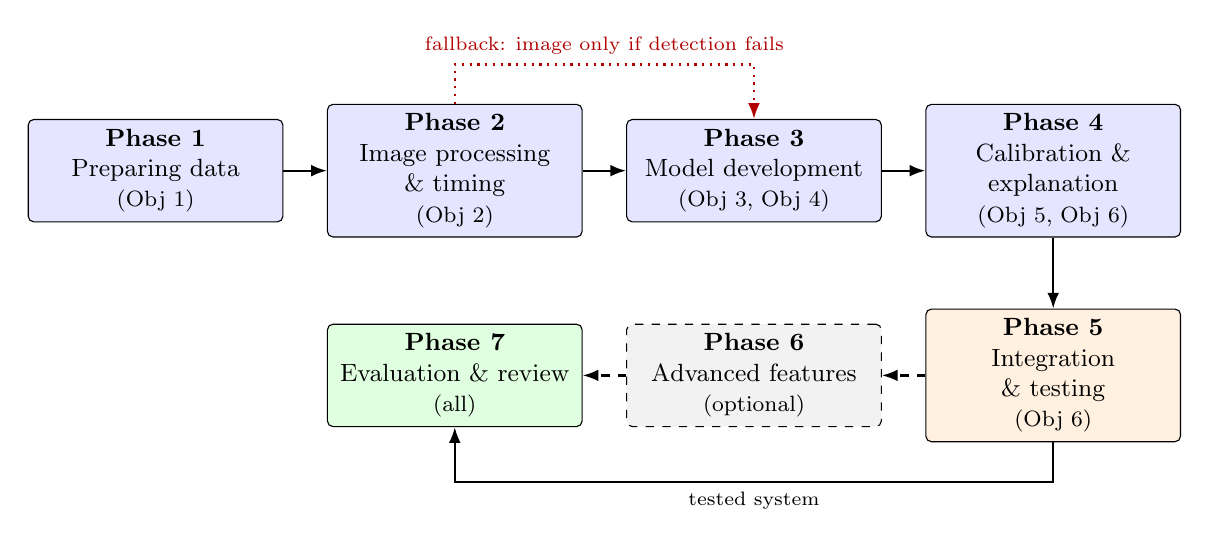
\begin{tikzpicture}[
      font=\small,
      phase/.style={draw, rounded corners=2pt, align=center, text width=30mm,
                    minimum height=13mm, fill=#1},
      phase/.default=blue!10,
      arr/.style={-{Latex[length=2mm]}, thick}
    ]
    \node[phase] (p1) at (0,0)     {\textbf{Phase 1}\\Preparing data\\\footnotesize(Obj 1)};
    \node[phase] (p2) at (38mm,0)  {\textbf{Phase 2}\\Image processing\\\& timing\\\footnotesize(Obj 2)};
    \node[phase] (p3) at (76mm,0)  {\textbf{Phase 3}\\Model development\\\footnotesize(Obj 3, Obj 4)};
    \node[phase] (p4) at (114mm,0) {\textbf{Phase 4}\\Calibration \& explanation\\\footnotesize(Obj 5, Obj 6)};
    \node[phase=orange!12] (p5) at (114mm,-26mm) {\textbf{Phase 5}\\Integration \& testing\\\footnotesize(Obj 6)};
    \node[phase=black!5, dashed] (p6) at (76mm,-26mm) {\textbf{Phase 6}\\Advanced features\\\footnotesize(optional)};
    \node[phase=green!12] (p7) at (38mm,-26mm) {\textbf{Phase 7}\\Evaluation \& review\\\footnotesize(all)};

    \draw[arr] (p1) -- (p2);
    \draw[arr] (p2) -- (p3);
    \draw[arr] (p3) -- (p4);
    \draw[arr] (p4) -- (p5);
    \draw[arr, dashed] (p5) -- (p6);
    \draw[arr, dashed] (p6) -- (p7);
    \draw[arr] (p5.south) -- ++(0,-5mm) -| node[pos=0.25, below, font=\scriptsize]{tested system} (p7.south);

    % fallback
    \draw[arr, dotted, red!70!black] (p2.north) -- ++(0,5mm) -| node[pos=0.25, above, font=\scriptsize]{fallback: image only if detection fails} (p3.north);
  \end{tikzpicture}%
  }
  \caption{Project workflow. Phase 6 is optional and is dropped first if the schedule slips.}
  \label{fig:workflow}
\end{figure}

\textbf{Phase 1: Preparing data (Obj 1).} Training images will be rendered from PTB-XL with ECG-Image-Kit, labelled with the nine classes and split by patient. A test set will be prepared from the PTB-XL part of the ECG-Image-Database, and the class counts recorded, as rare classes such as atrial flutter may need to be reported separately. As these real images are of PTB-XL recordings, their patients will be excluded from the training folds to prevent data leakage.

\textbf{Phase 2: Image processing and timing (Obj 2).} OpenCV will isolate the trace; R peaks, heart rate and RR regularity will then be measured and checked against Pan--Tompkins on the source signal. A quality check will warn the user when the trace cannot be found or the resolution is too low (FR15). If detection is unreliable on real images, the classifier will use the image alone.

\textbf{Phase 3: Model development (Obj 3, Obj 4).} A multi-label CNN will be trained on rendered images, with and without timing features, and a pretrained CNN fine-tuned on the same splits for comparison. Both will be evaluated per class on rendered and real images.

\textbf{Phase 4: Calibration and explanation (Obj 5, Obj 6).} Temperature scaling will be fitted on the validation fold, and Grad-CAM heatmaps checked against expected regions and for shortcuts such as attention on the grid or text.

\textbf{Phases 5--7: Integration, extensions and evaluation (Obj 6).} The modules will be combined into one Python application and tested against the requirements; if time is short, the interface will be reduced to uploading, flagging and the heatmap. Optional features (Phase 6) are dropped first if the schedule slips. The project will then be evaluated (Section~\ref{sec:eval}), including the user study under the approved ethics application, with an expert review as the fallback. The risks behind these fallbacks are in Table~\ref{tab:risks} (Appendix~\ref{app:risks}).

Figure~\ref{fig:pipeline} shows the processing pipeline that Phases 2--5 will build: the CNN will use the preprocessed image and the timing features to give a score for each class, temperature scaling will calibrate the scores, and Grad-CAM will produce a heatmap for each flagged class.

\begin{figure}[!htbp]
  \centering
  \makebox[\linewidth][c]{%
  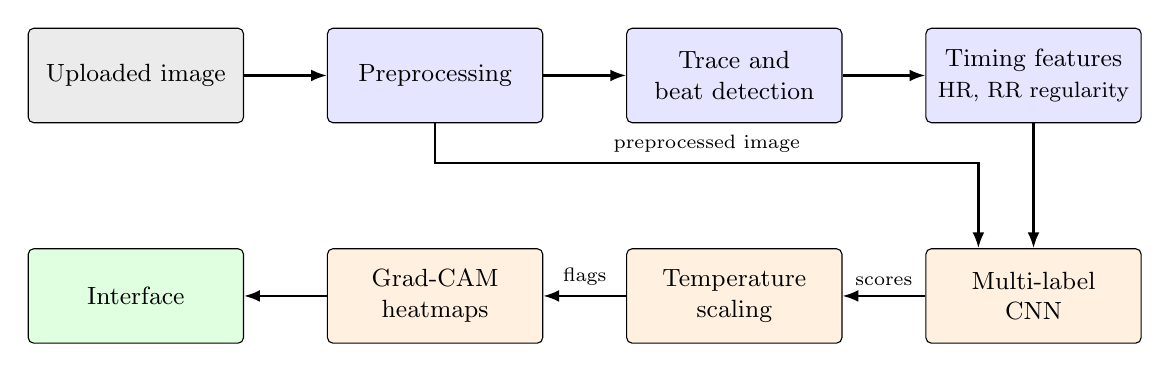
\begin{tikzpicture}[
      font=\small,
      step/.style={draw, rounded corners=2pt, align=center, text width=25mm,
                   minimum height=12mm, fill=#1},
      step/.default=blue!10,
      arr/.style={-{Latex[length=2mm]}, thick}
    ]
    \node[step=black!8] (up)  at (0,0)     {Uploaded image};
    \node[step]         (pre) at (38mm,0)  {Preprocessing};
    \node[step]         (det) at (76mm,0)  {Trace and beat detection};
    \node[step]         (tim) at (114mm,0) {Timing features\\\footnotesize HR, RR regularity};
    \node[step=orange!12] (cnn) at (114mm,-28mm) {Multi-label\\CNN};
    \node[step=orange!12] (cal) at (76mm,-28mm)  {Temperature scaling};
    \node[step=orange!12] (gc)  at (38mm,-28mm)  {Grad-CAM heatmaps};
    \node[step=green!12]  (ui)  at (0,-28mm)     {Interface};

    \draw[arr] (up) -- (pre);
    \draw[arr] (pre) -- (det);
    \draw[arr] (det) -- (tim);
    \draw[arr] (tim) -- (cnn);
    \draw[arr] (pre.south) -- ++(0,-5mm) -| node[pos=0.25, above, font=\scriptsize]{preprocessed image} ([xshift=-7mm]cnn.north);
    \draw[arr] (cnn) -- node[above, font=\scriptsize]{scores} (cal);
    \draw[arr] (cal) -- node[above, font=\scriptsize]{flags} (gc);
    \draw[arr] (gc) -- (ui);
  \end{tikzpicture}%
  }
  \caption{Planned processing pipeline, from an uploaded image to the results shown in the interface.}
  \label{fig:pipeline}
\end{figure}

\section{Testing and Evaluation Strategy}
\label{sec:evaluation}

Testing will verify that each requirement has been met; evaluation will assess the project against its aim, objectives and research questions.

\subsection{Testing}
\label{sec:testing}

Each module will be tested on its own before the integrated system. Every requirement is mapped to the module that implements it, its deliverable and a test case in the Requirements Traceability Matrix, given in Tables~\ref{tab:rtm-fr} and~\ref{tab:rtm-nfr} (Appendix~\ref{app:rtm}). The result column will record whether each requirement was met after system testing. Detection will be tested on images whose source signal is available: a detected R peak counts as correct if it lies within $\pm150$\,ms of the Pan--Tompkins peak on that signal \cite{pan_real-time_1985}, and the mean absolute errors of the heart rate and RR intervals will be reported.

\subsection{Evaluation}
\label{sec:eval}

Each objective will be marked as achieved, partly achieved or not achieved using the evidence in Table~\ref{tab:obj-eval}, the percentage achieved will be reported, and any shortfall explained.

\begin{table}[H]
  \centering
  \footnotesize
  \setlength{\arrayrulewidth}{0.8pt}
  \renewcommand{\arraystretch}{1.12}
  \caption{Evaluation of the objectives.}
  \label{tab:obj-eval}
  \begin{tabular}{|p{0.07\linewidth}|p{0.36\linewidth}|p{0.34\linewidth}|p{0.11\linewidth}|}
    \hline
    \rowcolor{cyan!90!black}
    \textcolor{white}{\textbf{Obj.}} & \textcolor{white}{\textbf{Evidence}} &
    \textcolor{white}{\textbf{Requirements and tests}} & \textcolor{white}{\textbf{Status}} \\
    \hline
    Obj 1 & Rendered training set and labelled real test set, with class counts & FR01; Phase 1 outputs & \\
    \hline
    Obj 2 & Preprocessing and detection results on rendered and real images & FR02--FR04, FR15; TC02--TC04, TC15 & \\
    \hline
    Obj 3 & Per-class sensitivity, specificity, MCC and AUROC & FR05, FR06, NFR02, NFR08; TC05, TC06, TC17, TC23 & \\
    \hline
    Obj 4 & Rendered-to-real gap per class & NFR04; TC19 & \\
    \hline
    Obj 5 & ECE and reliability diagrams before and after scaling & FR07, NFR03; TC07, TC18 & \\
    \hline
    Obj 6 & Heatmap checks, working GUI and user-study results & FR08--FR14, NFR01, NFR05, NFR06; TC08--TC16, TC20, TC21 & \\
    \hline
  \end{tabular}
\end{table}

\noindent\begin{minipage}{\linewidth}
\setlength{\parindent}{15pt}
\textbf{Experiments.} Models will be tested on the rendered PTB-XL test fold (folds 1--8 train, 9 validation, 10 test, split by patient) \cite{wagner_ptbxl_2020} and on real images from the ECG-Image-Database \cite{reyna_ecg-image-database_2024}, split by image type where numbers allow. Each class threshold will be chosen on the validation fold to maximise MCC (0.5 for classes with too few validation cases) and held fixed for all test sets, and each class scored by sensitivity, specificity, MCC and AUROC rather than accuracy, as the classes are imbalanced \cite{chicco_advantages_2020}. The rendered-to-real gap (SQ1) is the per-class difference in AUROC and MCC. Calibration (SQ2) will be measured per class by the ECE before and after temperature scaling, with reliability diagrams. The own CNN will be compared with the pretrained model, and with a variant without timing features, with bootstrap confidence intervals for small classes. For SQ3, heatmaps will be checked on labelled cases, and students will complete a questionnaire on their understanding of the confidence and heatmap, plus the SUS.
\end{minipage}

\textbf{Success criteria} are the targets in Table~\ref{tab:functional-req} (FR03, FR04 and NFR02--NFR05); the rendered-to-real gap will be reported whether or not its target is met, as it is a result in its own right. \textbf{Limitations:} labels come from at most two annotators and cardiologists can disagree \cite{wagner_ptbxl_2020,dhutia_interrater_2017}, and PTB-XL reflects one period and manufacturer. The wider issues are discussed in Appendix~\ref{app:ples}.
	\chapter{Feasibility}
\label{ch:feasibility}

This chapter shows that the plan in Chapter~\ref{ch:method} is achievable, through the planned environment, the datasets, the system design and the prototypes built so far.

\section{Coding Environment}
\label{sec:env}

The system will be developed in Python. OpenCV \cite{bradski_opencv_2000} will be used for image processing, PyTorch for the networks and Grad-CAM, and matplotlib for the interface; these were chosen for their mature libraries and their support for displaying ECG images and plots. Training will run on my own PC, which has a GPU, and the code will be kept under version control on GitHub (Appendix~\ref{app:repo}).

\section{Datasets}
\label{sec:datasets}

\begin{table}[H]
  \centering
  \footnotesize
  \begin{minipage}[t]{0.40\linewidth}
    \vspace{0pt}
    \centering
    \caption{Records per class in PTB-XL.}
    \label{tab:class-counts}
    \begin{tabular}{@{}lr@{}}
      \toprule
      \textbf{Class} & \textbf{Records} \\
      \midrule
      Normal & 9514 \\
      Myocardial infarction & 5469 \\
      ST/T change & 5235 \\
      Conduction disturbance & 4898 \\
      Hypertrophy & 2649 \\
      Atrial fibrillation & 1514 \\
      Atrial flutter & 73 \\
      Sinus tachycardia & 826 \\
      Sinus bradycardia & 637 \\
      \bottomrule
    \end{tabular}
  \end{minipage}\hfill
  \begin{minipage}[t]{0.55\linewidth}
    \vspace{0pt}
    \normalsize
    PTB-XL provides 21,800 labelled twelve-lead ECGs with patient-wise folds \cite{wagner_ptbxl_2020}; Table~\ref{tab:class-counts} gives the records per class. The ECG-Image-Database provides 35,595 real images of 1,977 recordings, 977 from PTB-XL and 1,000 from Emory Healthcare \cite{reyna_ecg-image-database_2024}. The PTB-XL part can be matched to PTB-XL labels by record, giving the labelled real test set; real images per class, and whether the Emory labels map to the nine classes, will be checked in Phase 1. Because the real images are of PTB-XL recordings, their patients will be removed from the training folds, so that no ECG is seen in both training and testing. Rare classes may only be evaluated on rendered images.
  \end{minipage}
\end{table}

\section{Design}
\label{sec:design}

Figure~\ref{fig:architecture} shows the architecture, with each module's inputs and outputs. The modules will be separate, so any one can be replaced without changing the others (NFR10). The GUI will offer a user view, with explanations, and a clinical view, with every class score, its threshold and fuller measured values. Offline training will produce the model weights, temperature $T$ and class thresholds that the application loads.

\begin{figure}[H]
  \centering
  \makebox[\linewidth][c]{%
  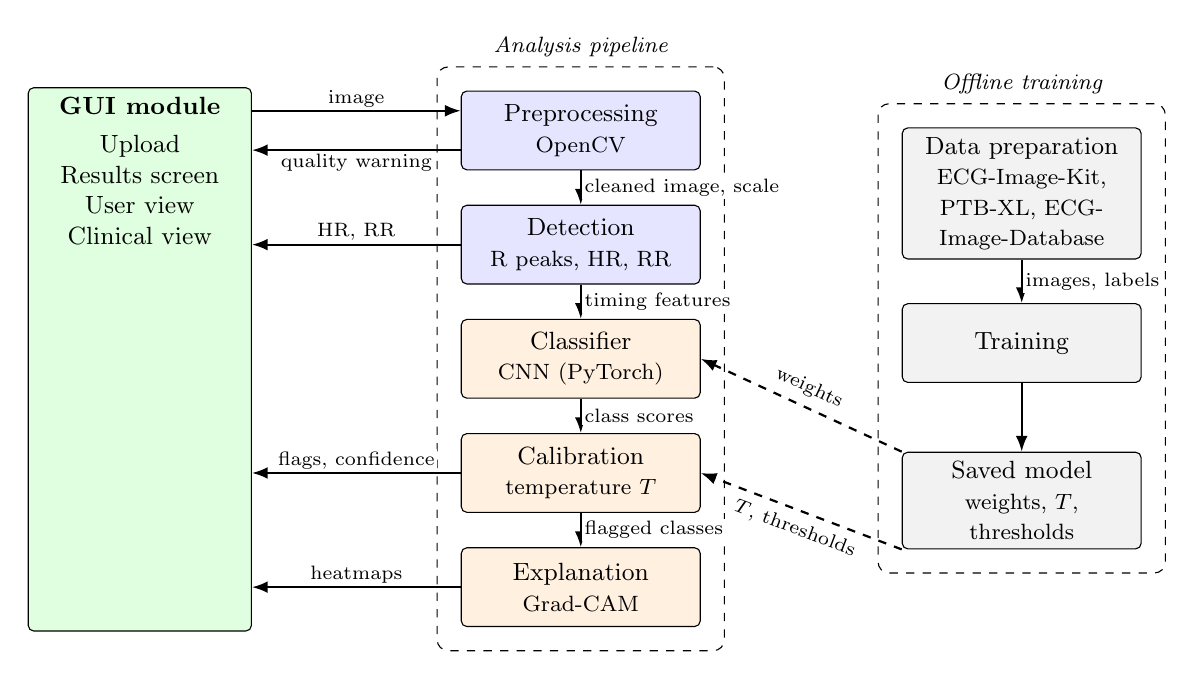
\begin{tikzpicture}[
      font=\small,
      mod/.style={draw, rounded corners=2pt, align=center, text width=28mm,
                  minimum height=10mm, fill=#1},
      mod/.default=blue!10,
      arr/.style={-{Latex[length=2mm]}, thick},
      lab/.style={font=\scriptsize, fill=white, inner sep=1pt}
    ]
    % analysis pipeline (middle column)
    \node[mod] (pre) at (0,0)      {Preprocessing\\\footnotesize OpenCV};
    \node[mod] (det) at (0,-14.5mm)  {Detection\\\footnotesize R peaks, HR, RR};
    \node[mod=orange!12] (clf) at (0,-29mm) {Classifier\\\footnotesize CNN (PyTorch)};
    \node[mod=orange!12] (cal) at (0,-43.5mm) {Calibration\\\footnotesize temperature $T$};
    \node[mod=orange!12] (exp) at (0,-58mm) {Explanation\\\footnotesize Grad-CAM};
    \node[draw, dashed, rounded corners, inner sep=3mm, fit=(pre)(exp),
          label={[font=\footnotesize\itshape]above:Analysis pipeline}] (pipe) {};

    % GUI (left)
    \node[mod=green!12, minimum height=69mm, text width=26mm, anchor=north]
         (gui) at (-56mm,5.5mm) {};
    \node[align=center, font=\small, text width=24mm, anchor=north] at (gui.north)
         {\textbf{GUI module}\\[3pt]Upload\\Results screen\\User view\\Clinical view};

    % offline training (right)
    \node[mod=black!5] (data) at (56mm,-8mm) {Data preparation\\\footnotesize ECG-Image-Kit, PTB-XL, ECG-Image-Database};
    \node[mod=black!5] (train) at (56mm,-27mm) {Training};
    \node[mod=black!5] (store) at (56mm,-47mm) {Saved model\\\footnotesize weights, $T$, thresholds};
    \node[draw, dashed, rounded corners, inner sep=3mm, fit=(data)(store),
          label={[font=\footnotesize\itshape]above:Offline training}] {};

    % pipeline flow
    \draw[arr] (pre) -- node[lab, right]{cleaned image, scale} (det);
    \draw[arr] (det) -- node[lab, right]{timing features} (clf);
    \draw[arr] (clf) -- node[lab, right]{class scores} (cal);
    \draw[arr] (cal) -- node[lab, right]{flagged classes} (exp);

    % GUI <-> pipeline
    \draw[arr] (gui.east |- 0,2.5mm) -- node[lab, above]{image} ([yshift=2.5mm]pre.west);
    \draw[arr] ([yshift=-2.5mm]pre.west) -- node[lab, below]{quality warning} (gui.east |- 0,-2.5mm);
    \draw[arr] (det.west) -- node[lab, above]{HR, RR} (gui.east |- det);
    \draw[arr] (cal.west) -- node[lab, above]{flags, confidence} (gui.east |- cal);
    \draw[arr] (exp.west) -- node[lab, above]{heatmaps} (gui.east |- exp);

    % offline flow
    \draw[arr] (data) -- node[lab, right]{images, labels} (train);
    \draw[arr] (train) -- (store);
    \draw[arr, dashed] (store.north west) -- node[font=\scriptsize, above, sloped, pos=0.5]{weights} (clf.east);
    \draw[arr, dashed] (store.south west) -- node[font=\scriptsize, below, sloped, pos=0.5]{$T$, thresholds} (cal.east);
  \end{tikzpicture}%
  }
  \caption{Planned system architecture, showing the modules, their inputs and outputs, and how they connect.}
  \label{fig:architecture}
\end{figure}

\section{Prototypes}
\label{sec:prototypes}

Three prototypes test the main risks of the plan. Table~\ref{tab:prototypes} gives the status of each one and what it demonstrates, Figures~\ref{fig:rendered} and~\ref{fig:proto2} show the first two, and the wireframes are in Appendix~\ref{app:wireframes}.

\begin{table}[H]
  \centering
  \footnotesize
  \setlength{\arrayrulewidth}{0.8pt}
  \renewcommand{\arraystretch}{1.15}
  \caption{Status of the prototypes.}
  \label{tab:prototypes}
  \begin{tabular}{|p{0.22\linewidth}|p{0.12\linewidth}|p{0.56\linewidth}|}
    \hline
    \rowcolor{cyan!90!black}
    \textcolor{white}{\textbf{Prototype}} & \textcolor{white}{\textbf{Status}} &
    \textcolor{white}{\textbf{Demonstrates}} \\
    \hline
    1: Data and rendering & Completed & PTB-XL labels were mapped to the nine classes, and records were rendered with ECG-Image-Kit. The rendered beats match the source signal's timing, but the trace is cleaner than real images, which supports measuring the rendered-to-real gap. \\
    \hline
    2: Preprocessing & Completed & OpenCV thresholding removed colour and separated the trace, and feature detection removed the grid, leaving the trace alone. Beat detection is planned for Phase 2. \\
    \hline
    3: GUI wireframes & Completed & Show the user and clinical views, and how flags, confidence, heatmaps and measured values are presented, before the interface is built (Appendix~\ref{app:wireframes}). \\
    \hline
  \end{tabular}
\end{table}

\begin{figure}[H]
  \centering
  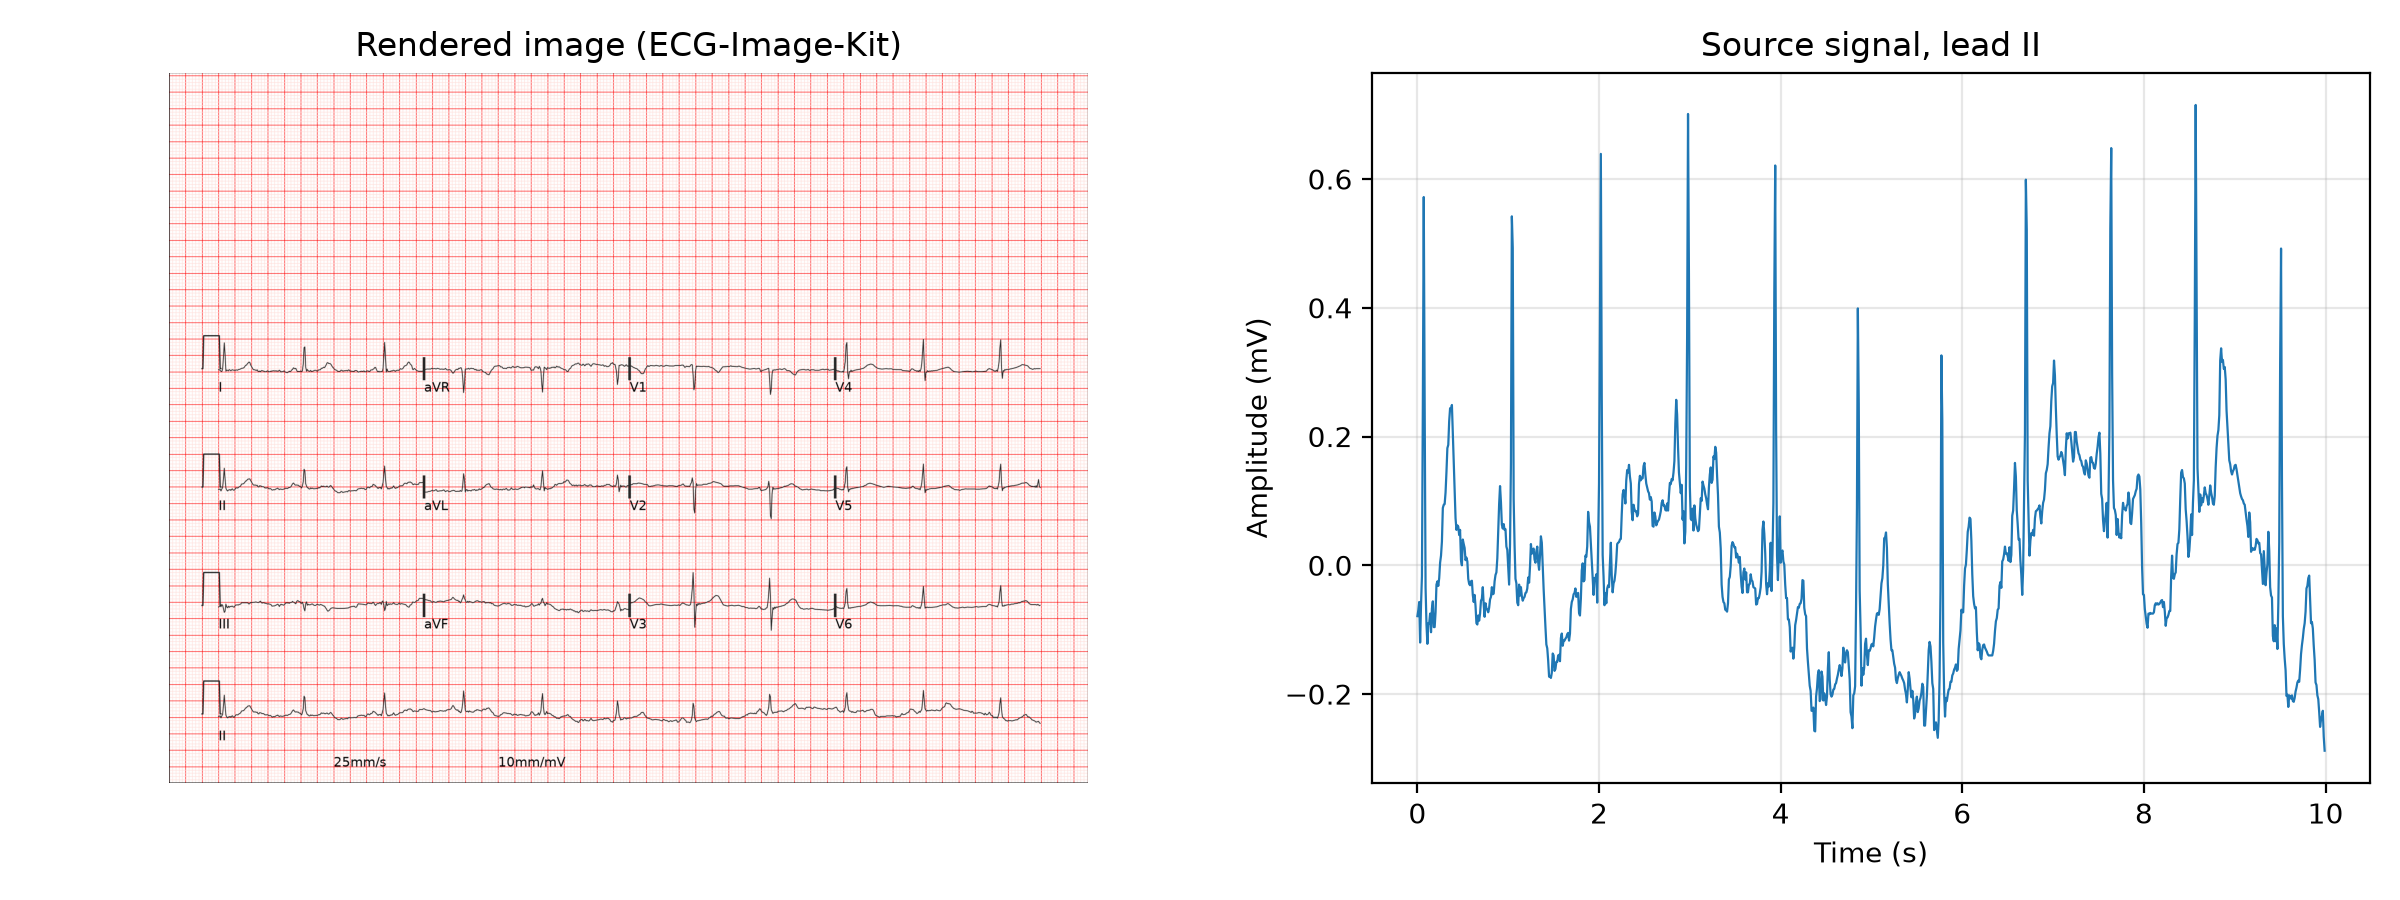
\includegraphics[width=0.85\linewidth,height=0.22\textheight,keepaspectratio]{images/rendered_vs_signal.png}
  \caption{Prototype 1: PTB-XL record 00001\_lr rendered with ECG-Image-Kit
    \cite{shivashankara_ecg-image-kit_2024} (left), and the lead II signal it was generated
    from (right). Both show 11 beats at about 0.9--1.0\,s spacing.}
  \label{fig:rendered}
\end{figure}

\begin{figure}[H]
  \centering
  \begin{subfigure}[b]{0.35\linewidth}
    \centering
    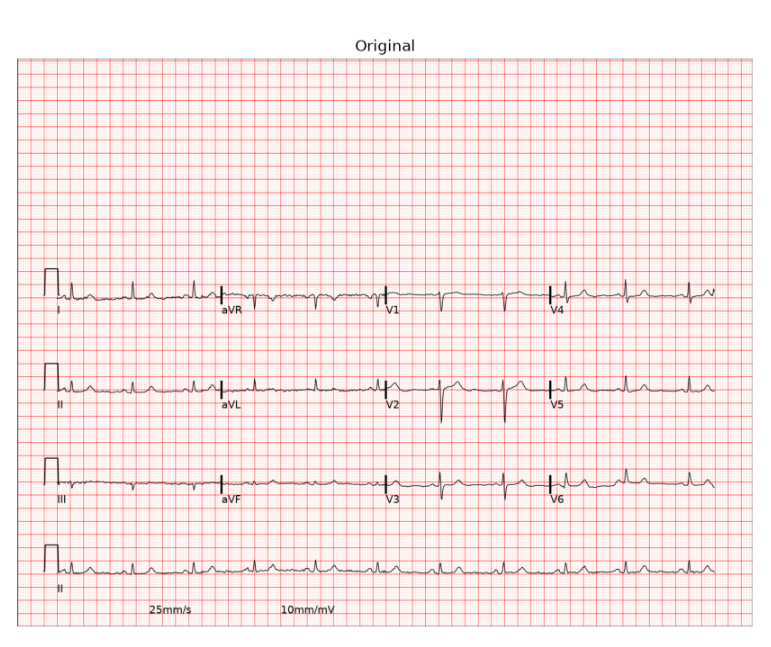
\includegraphics[width=\linewidth]{images/p2_initial.png}
    \caption{Initial Image.}
    \label{fig:img1}
  \end{subfigure}\hfill
  \begin{subfigure}[b]{0.35\linewidth}
    \centering
    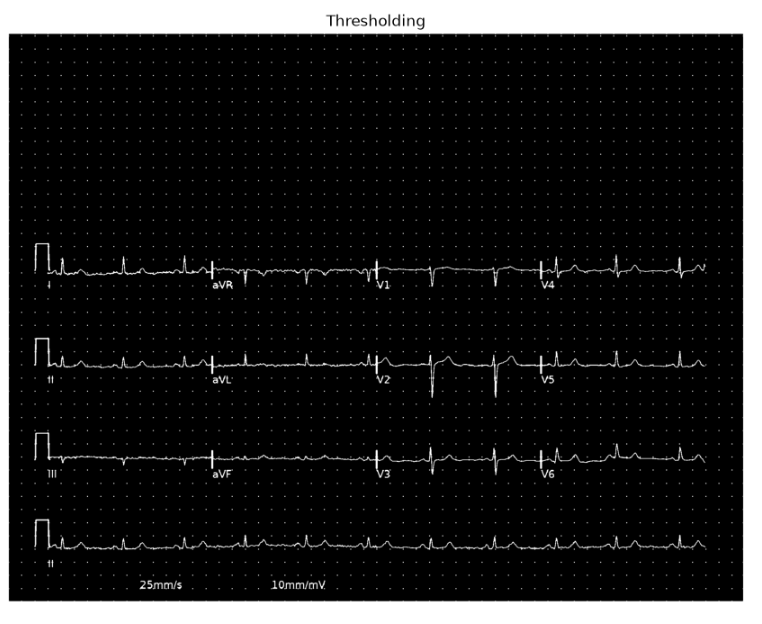
\includegraphics[width=\linewidth]{images/p2_thre.png}
    \caption{Image thresholded.}
    \label{fig:img2}
  \end{subfigure}\hfill
  \begin{subfigure}[b]{0.35\linewidth}
    \centering
    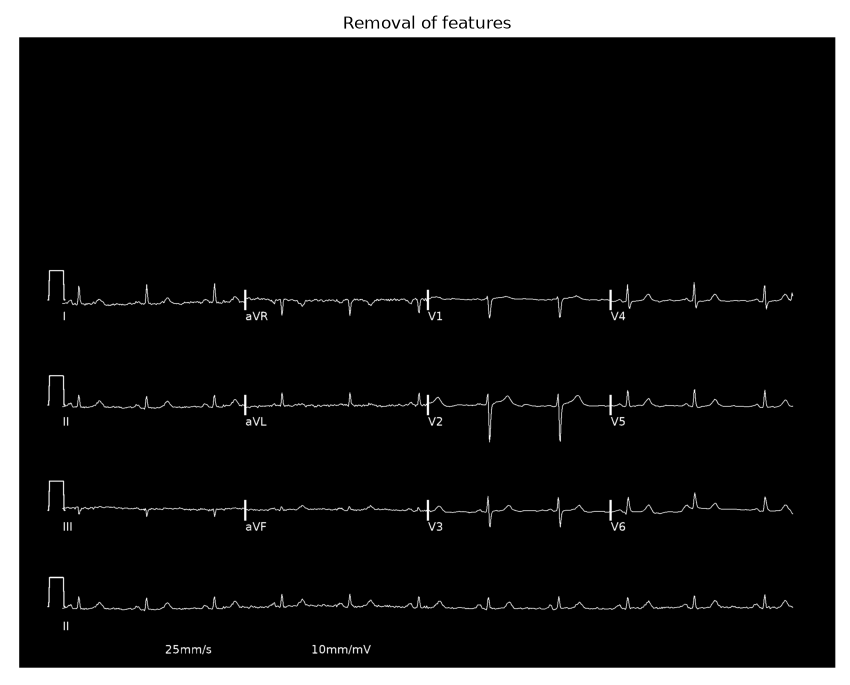
\includegraphics[width=\linewidth]{images/p2_remov.png}
    \caption{Features Removed.}
    \label{fig:img3}
  \end{subfigure}
  \caption{Extracting a waveform from an ECG.}
  \label{fig:proto2}
\end{figure}
\section{Risks}
\label{sec:feas-risks}

The full risk assessment is in Table~\ref{tab:risks} (Appendix~\ref{app:risks}). The main risks for feasibility are that models may not transfer from rendered to real images (R1), that detection may fail on poor images (R2), that rare classes have too few cases (R3), and that time may run short for the full interface (R10). Their fallbacks are reporting the gap as a result, classifying from the image alone, reporting rare classes with counts, and a reduced interface.
	\chapter{Conclusion}
\label{ch:conc}

\section{Summary}
\label{sec:conc-summary}

This project will build and evaluate a CNN application that flags possible abnormalities in ECG images, reports calibrated confidence, and explains its predictions to different users. It will train on images rendered from PTB-XL and test on real images, addressing four gaps in the literature: limited testing on real images, missing calibration, unevaluated explanations, and little evidence on presenting results to different users.

The work is organised into seven phases (Section~\ref{sec:dev-plan}), with requirements tested through the Requirements Traceability Matrix and the project evaluated against its objectives, including a user study under the approved ethics application. Two prototypes, rendering and preprocessing, are complete, and GUI wireframes are planned. The main risks are the rendered-to-real gap, unreliable detection on poor images, and rare classes, and each has a fallback in the plan (Appendix~\ref{app:risks}).

\section{Expected Contributions}
\label{sec:contributions}

The project is expected to contribute three things beyond a working application:
\begin{enumerate}\setlength{\itemsep}{0pt}\setlength{\parskip}{0pt}
  \item \textbf{A per-class measure of the rendered-to-real gap.} Training on rendered images and testing on real ones of the same recordings, with leakage removed, will show which classes transfer to real images and which do not, and whether timing features reduce the gap (SQ1).
  \item \textbf{Calibration under data shift for a multi-label image classifier.} Measuring the calibration error per class before and after temperature scaling, on both rendered and real images, will show whether confidence scores fitted on rendered images can still be trusted on real ones (SQ2).
  \item \textbf{Evidence on presenting results to non-expert users.} The user study will show whether students can interpret calibrated confidence and Grad-CAM heatmaps, which few studies have evaluated with users (SQ3).
\end{enumerate}

\section{Next Steps}
\label{sec:next-steps}
 Semester 2 will follow the gantt schedule (Table~\ref{fig:gantt-s2}) in Appendix~\ref{app:gantt}. The first few weeks will render the full training set, match the real images to their labels and remove their patients from the training folds, and build the detection step, as every later phase depends on these. CNN training will then follow, with the GUI developed in parallel to it, aiming for a working prototype by week 9. The user study and evaluation will take place in weeks 9--11, leaving the final weeks for writing the dissertation. If the schedule slips, the fallbacks in Section~\ref{sec:dev-plan} will be applied in order, starting with dropping the optional features of Phase 6.
	\appendix
	

\chapter{Project Management}

\renewcommand{\thefigure}{A.\arabic{figure}}
\section{Risk Assessment and Mitigation}
\label{app:risks}

Table~\ref{tab:risks} gives the full risk assessment. Each risk is rated once for its likelihood and its severity, and lists every mitigation planned for it. Section~\ref{sec:feas-risks} refers to the risks most relevant to feasibility by their IDs.

\begingroup
\footnotesize
\renewcommand{\arraystretch}{1.2}
\begin{longtable}{|p{0.05\linewidth}|p{0.24\linewidth}|p{0.11\linewidth}|p{0.10\linewidth}|p{0.35\linewidth}|}
  \caption{Risk assessment and mitigation.}
  \label{tab:risks} \\
    \hline
    \textbf{ID} & \textbf{Risk} & \textbf{Likelihood} & \textbf{Severity} & \textbf{Mitigation} \\
    \hline
  \endfirsthead
    \multicolumn{5}{l}{\footnotesize\itshape Table~\ref{tab:risks} continued} \\
    \hline
    \textbf{ID} & \textbf{Risk} & \textbf{Likelihood} & \textbf{Severity} & \textbf{Mitigation} \\
    \hline
  \endhead
    \multicolumn{5}{|l|}{\textbf{Technical risks}} \\
    \hline
    R1 & A model trained on rendered images may not work on real images. & \High & \High &
      Generate a large training set with ECG-Image-Kit, and add augmentation that imitates real artefacts. Evaluate on real images and report the gap as a result. \\
    \hline
    R2 & Trace detection fails on poor-quality real images. & \Med & \Med &
      Evaluate detection separately on real images. If it is too unreliable, the CNN uses the image alone, and the failure is reported. \\
    \hline
    R3 & Some classes have too few examples to train a model. & \High & \Med &
      Report results per class with counts and bootstrap confidence intervals. Rare classes such as atrial flutter may be combined with atrial fibrillation, or evaluated on rendered images only. \\
    \hline
    R4 & Class imbalance biases the model towards the majority class. & \High & \Med &
      Use class weights to balance the loss function, and imbalance-aware metrics (sensitivity, specificity, MCC, AUROC). Choose a threshold for each class on the validation fold. \\
    \hline
    R5 & The ECG-Image-Database has very few images for some classes. & \High & \Med &
      Evaluate only the classes with enough real images; report the rest as a limitation. \\
    \hline
    R6 & Labels are subjective and may be inconsistent. & \Med & \Med &
      Use the PTB-XL validation and test folds, whose labels were checked to a higher standard, and report label quality as a limitation. \\
    \hline
    R7 & Heatmaps may be misleading. & \Med & \Med &
      Check heatmaps against known cases and for shortcuts; mask the grid if needed; evaluate the heatmaps in the user study. \\
    \hline
    R8 & The CNN underperforms. & \Med & \Med &
      Fine-tune a pretrained model on the same splits for comparison, and use it as the main model if it performs better. \\
    \hline
    R9 & Training is too slow. & \Low & \Low &
      Use smaller models or a lower image resolution to reduce the cost. \\
    \hline
    \multicolumn{5}{|l|}{\textbf{Project and ethical risks}} \\
    \hline
    R10 & The scope is too large for the time available, including the full interface. & \Med & \Med &
      Prioritise requirements with MoSCoW so that the most important are implemented first. Reduce the interface to uploading, flagging and the heatmap if time is short. \\
    \hline
    R11 & There are not enough participants for the user study. & \Med & \Med &
      Start recruitment early. If this fails, an expert review replaces the study. \\
    \hline
    R12 & Clinicians are not able to take part. & \High & \Low &
      Base the requirements on published studies of clinicians. State the limitation, and describe clinician testing as future work. \\
    \hline
    R13 & Software problems, such as package conflicts. & \Med & \Low &
      Use version control, and a virtual environment with a recorded list of package versions. \\
    \hline
    R14 & Loss of code or data. & \Low & \High &
      Keep remote copies on GitHub and regular backups of results (Section~\ref{app:repo}). \\
    \hline
    R15 & The user study goes beyond its approved ethical scope. & \Low & \High &
      Keep the study within the approved scope. Process images locally, and destroy participant data on completion of the project. \\
    \hline
    R16 & A dataset or tool update changes its availability or licence. & \Low & \Low &
      Keep local copies of the datasets; check and cite their licences. \\
    \hline
    R17 & The author cannot complete the project due to illness or other personal reasons. & \Low & \High &
      Plan the project with deadlines, and keep the supervisor informed of progress. \\
    \hline
\end{longtable}
\endgroup
\section{PLES}
\label{app:ples}


This section considers the professional, legal, ethical and social issues that this project raises. The project is a research prototype, that analyses ECG images and presents results to students and other users. It is not supposed to be for clinical use.
\subsection{Professional Issues}
The project follows the BCS Code of Conduct. These are the principles that apply most directly:

\begin{itemize}
  \item Public interest means that results are reported with honesty, even if they do not support my claim fully.  
  \item All datasets, tools, and papers used are cited.
  \item The preliminary results are described as pilot results.
  \item The use of generative AI is declared in the GenAI summary.
  \item All code is kept under version control
  \item Coding environment and its data is documented, so results can be reproduced.
\end{itemize}

\subsection{Legal Issues}
As ECG data is considered medical data, the UK Data Protection Law treats this as special category data. The training data comes from public, anonymised datasets, so the project does not process patient records that can be identified. The user study will still collect questionnaire responses, but they will be kept anonymous, and deleted upon project completion. Images uploaded to the interface are processed on the local machine, and will not be stored beyond the session.

Software that is intended to support clinically can be regulated as a medical device. This project is an academic prototype, and so will not be placed on markets or used on patients. This has been stated as such. Any later clinical use would need regulation, a clinical safety assessment, and validation on more data than the project uses.
PTB-XL and ECG-Image-Database are released under CC BY 4.0, whilst ECG-Image-Kit is under BSD 3-Clause License. They are cited whenever they are used, and the images generated by the toolkit are used under these terms. Figures from other sources are reproduced with a citation, and figures that the author produces are labelled as such. Copyright in the code, and the report, belong to the author under the university's regulations. 

\subsection{Ethical Issues}
The project will have ethical approval. Participants in the user study will give informed consent, in addition to be able to withdraw at any time, and are also not asked personal or health information.

The main risk of a tool that flags abnormalities is that users may rely on it. False negatives or positives can cause unecessary worry. Automation bias is documented in computer-interpreted ECGs. Inexperienced
users may accept an automated reading without question,
and explanations can raise the trust of novices more than experts. The project therefore reports a calibrated confidence for each
class so that any uncertainty is shown. It also checks heatmaps against known cases, and presents the
tool as a learning and research aid whose output has to be checked by a person.
Users are told how the model was trained, and where its weaknesses are.

\subsection{Social Issues}
As PTB-XL was collected 40 years ago, patient recording are limited. A model trained on this may perform differently for other populations, and so the project is not able to test this. The report does not claim that the results would hold on another system.

The tool could help students learn about ECG interpretation, and systems that read ECG images could widen the access to automated analysis, where only paper records exist. In addition, the interface should be usable by people with different needs, and any explanations should be clear and simple. However, users that over-rely on the tool may learn less information. Therefore, it is designed to explain the reasoning, to support learning.

For the environment, training deep models use a lot of energy. The project limits this using a small model, and pretrained weight if possible.
\section{GenAI Summary}
\label{app: genai}
Generative AI was used for LaTex debugging, and grammatical as well as spelling errors. It was also used to help with formatting certain parts of the structure, but all the written body is in my own words. Every reference and citation I have found without the use of generative ai.

\section{Repository Management}
\label{app:repo}

The project's code will be kept in a private GitHub repository, with a working copy on the development PC. The repository will be organised by module, matching the architecture in Section~\ref{sec:design}: separate folders for data preparation scripts, preprocessing, detection, models, calibration and explanation, the GUI, experiment configurations, and tests.

\textbf{Data and large files.} The datasets (PTB-XL and the ECG-Image-Database) and the rendered images are too large to store in Git, and are distributed under their own licences, so they will be excluded with a \texttt{.gitignore} file. The repository will instead contain the scripts that download the datasets and render the images, so that they can be recreated (NFR08). Trained model weights will also be stored outside Git.

\textbf{Branching and commits.} The \texttt{main} branch will always hold a working version. New work will be done on a separate branch for each phase or feature, and merged into \texttt{main} once its tests pass. Commits will be small, with descriptive messages, and each milestone (D1, the working prototype and the final submission) will be tagged so that it can be recovered.

\textbf{Reproducibility.} The Python environment will be recorded in a \texttt{requirements.txt} file with pinned package versions, and each experiment will have a configuration file recording its settings and random seed, so that the reported results can be regenerated from a fresh clone (NFR08, TC23).

\textbf{Backups.} GitHub will act as the remote copy of the code. Results, model weights and the report will be backed up weekly to the university OneDrive (R14).

\section{Gantt Chart}
\label{app:gantt}
\begin{figure}[H]
  \centering
  \makebox[\linewidth][c]{%
  \begin{ganttchart}[
      hgrid,
      vgrid={*1{black!25, dotted}},
      x unit=1.0cm,
      y unit title=0.9cm,
      y unit chart=0.9cm,
      time slot format=simple,
      title label font=\normalsize\bfseries,
      bar label font=\large,
      group label font=\large\bfseries,
      milestone label font=\large\itshape,
      bar height=0.55,
      bar/.append style={fill=blue!30},
      group/.append style={fill=black!70},
      milestone/.append style={fill=red!60},
      link/.style={-latex, thick, black!60}
    ]{1}{12}

    \gantttitle{Week}{12} \\
    \gantttitlelist{1,...,12}{1} \\

    \ganttgroup{D1 report}{1}{11} \\
    \ganttbar[name=supervisor]{Supevisor Selection}{1}{3} \\
    \ganttbar[name=topic]{Topic Selection}{1}{3} \\
    \ganttbar[name=abs]{Abstract}{3}{3} \\
    \ganttbar[name=intro]{Introduction}{3}{4} \\
    \ganttbar[name=lit]{Literature review}{4}{7} \\
    \ganttbar[name=meth]{Methodology}{7}{8} \\
    \ganttbar[name=req]{Requirements}{8}{8} \\
    \ganttbar[name=pp]{Project Plan}{8}{9} \\
    \ganttbar[name=feasi]{Feasibility}{9}{10} \\
    \ganttbar[name=conc]{Conclusion}{10}{10} \\
    \ganttbar[name=prt]{Prototypes}{9}{11} \\
    \ganttbar[name=appe]{Appendix}{3}{11} \\
    \ganttbar[name=ethics]{Ethics form}{3}{7} \\
    \ganttmilestone[name=esub]{Ethics Submission}{7} \\
    \ganttmilestone[name=dsub]{D1 and D2 submission}{11} \\

    \ganttlink{topic}{abs}
    \ganttlink{abs}{intro}
  
    \ganttlink{intro}{lit}
    \ganttlink{lit}{meth}
    \ganttlink{meth}{req}
    \ganttlink{req}{pp}
    \ganttlink{pp}{feasi}
    \ganttlink{feasi}{conc}
    \ganttlink{conc}{prt}
    \ganttlink{appe}{dsub}
    \ganttlink{ethics}{esub}
  \end{ganttchart}%
  }
  \caption{Project plan for Semester 1.}
  \label{fig:gantt-s1}
\end{figure}
\clearpage

% ================= Semester 2 =================
\begin{figure}[H]
  \centering
  \makebox[\linewidth][c]{%
  \begin{ganttchart}[
      hgrid,
      vgrid={*1{black!25, dotted}},
      x unit=1.25cm,
      y unit title=0.9cm,
      y unit chart=1.1cm,
      time slot format=simple,
      title label font=\normalsize\bfseries,
      bar label font=\large,
      group label font=\large\bfseries,
      milestone label font=\large\itshape,
      bar height=0.55,
      bar/.append style={fill=blue!30},
      group/.append style={fill=black!70},
      milestone/.append style={fill=red!60},
      link/.style={-latex, thick, black!60}
    ]{1}{12}

    \gantttitle{Week}{12} \\
    \gantttitlelist{1,...,12}{1} \\

    \ganttgroup{Implementation}{1}{11} \\
    \ganttbar[name=env]{Environment Setup}{1}{1} \\
    \ganttbar[name=img-gen]{Image generation}{2}{2} \\
    \ganttbar[name=pre]{Preprocessing}{3}{3} \\
    \ganttbar[name=cnn-creat]{CNN creation}{4}{5} \\
    \ganttbar[name=cnn-train]{CNN training}{5}{7} \\
    \ganttbar[name=heat]{Heatmaps}{7}{7} \\
    \ganttbar[name=exp]{Explanations}{8}{8} \\
    \ganttbar[name=gui]{GUI development}{4}{9} \\
    \ganttmilestone[name=proto]{Working prototype}{9} \\
    \ganttbar[name=study]{User study}{9}{11} \\
    \ganttbar[name=eval]{Evaluation \& results}{10}{11} \\
    \ganttbar[name=d3]{Dissertation writing}{6}{11} \\
    \ganttmilestone[name=d3sub]{Final submission}{11} \\

    \ganttlink{env}{img-gen}
    \ganttlink{img-gen}{pre}
    \ganttlink{pre}{cnn-creat}
    \ganttlink{cnn-creat}{cnn-train}
    \ganttlink{cnn-train}{heat}
    \ganttlink{heat}{exp}
    \ganttlink{gui}{proto}
    \ganttlink{exp}{proto}
    \ganttlink{proto}{study}
    \ganttlink{study}{eval}
    \draw[-latex, thick, black!60] (eval.east) -- (d3sub.north); % Added to stop overlapping
    \draw[-latex, thick, black!60] (d3.east) -- (d3sub.north);
  \end{ganttchart}%
  }
  \caption{Project plan for Semester 2.}
  \label{fig:gantt-s2}
\end{figure}
\clearpage
\chapter{Wireframes}
\label{app:wireframes}

\begin{figure}[H]
  \centering
  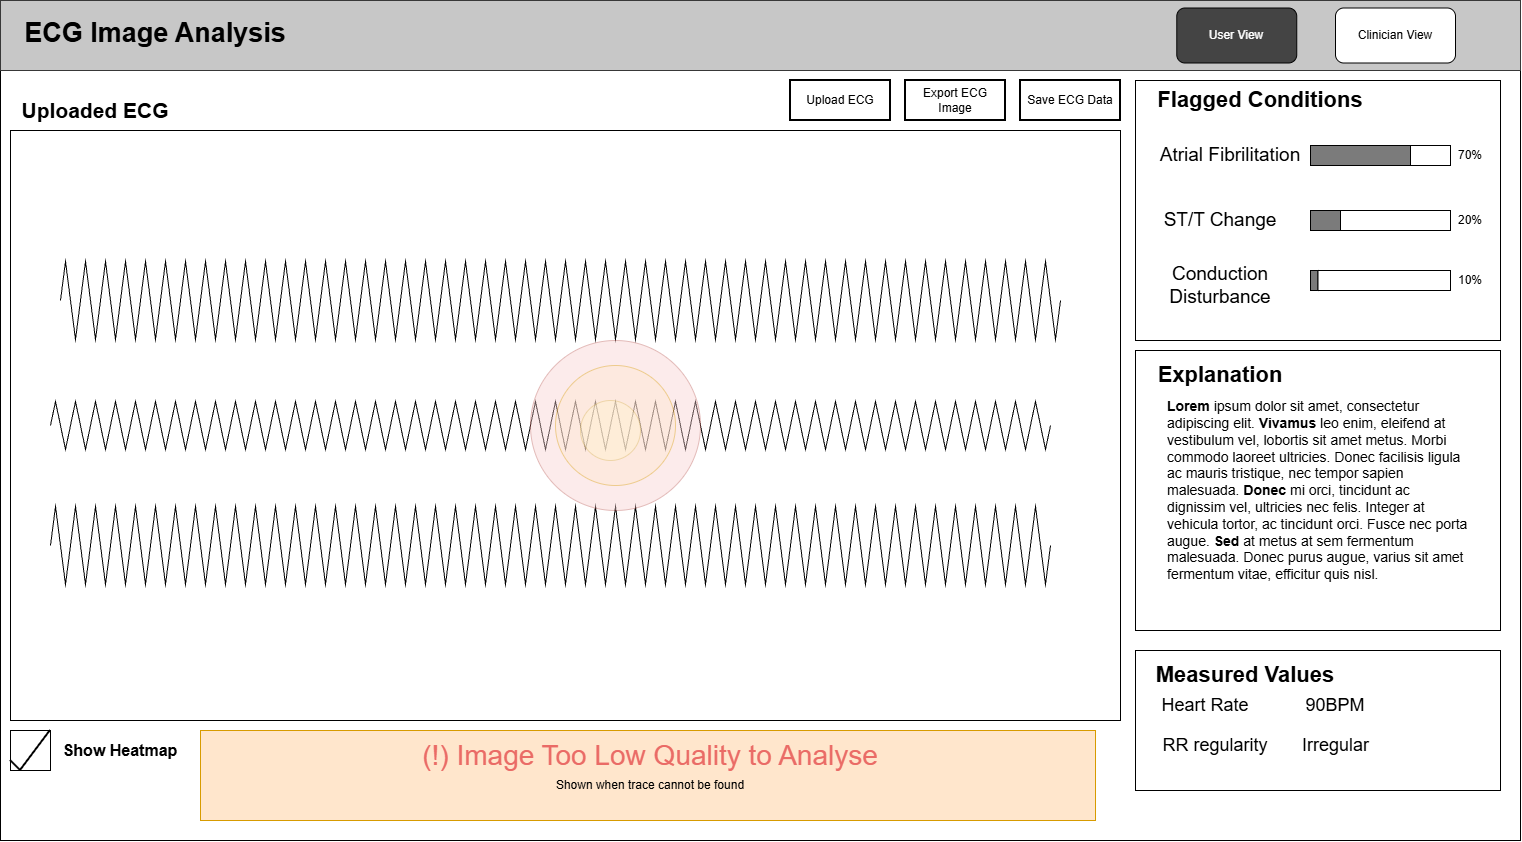
\includegraphics[width=0.85\linewidth,height=0.5\textheight,keepaspectratio]{images/user_view.png}
  \caption{Prototype 3: Wireframe created of the user view.}
  \label{fig:proto3user}
\end{figure}

\begin{figure}[H]
  \centering
  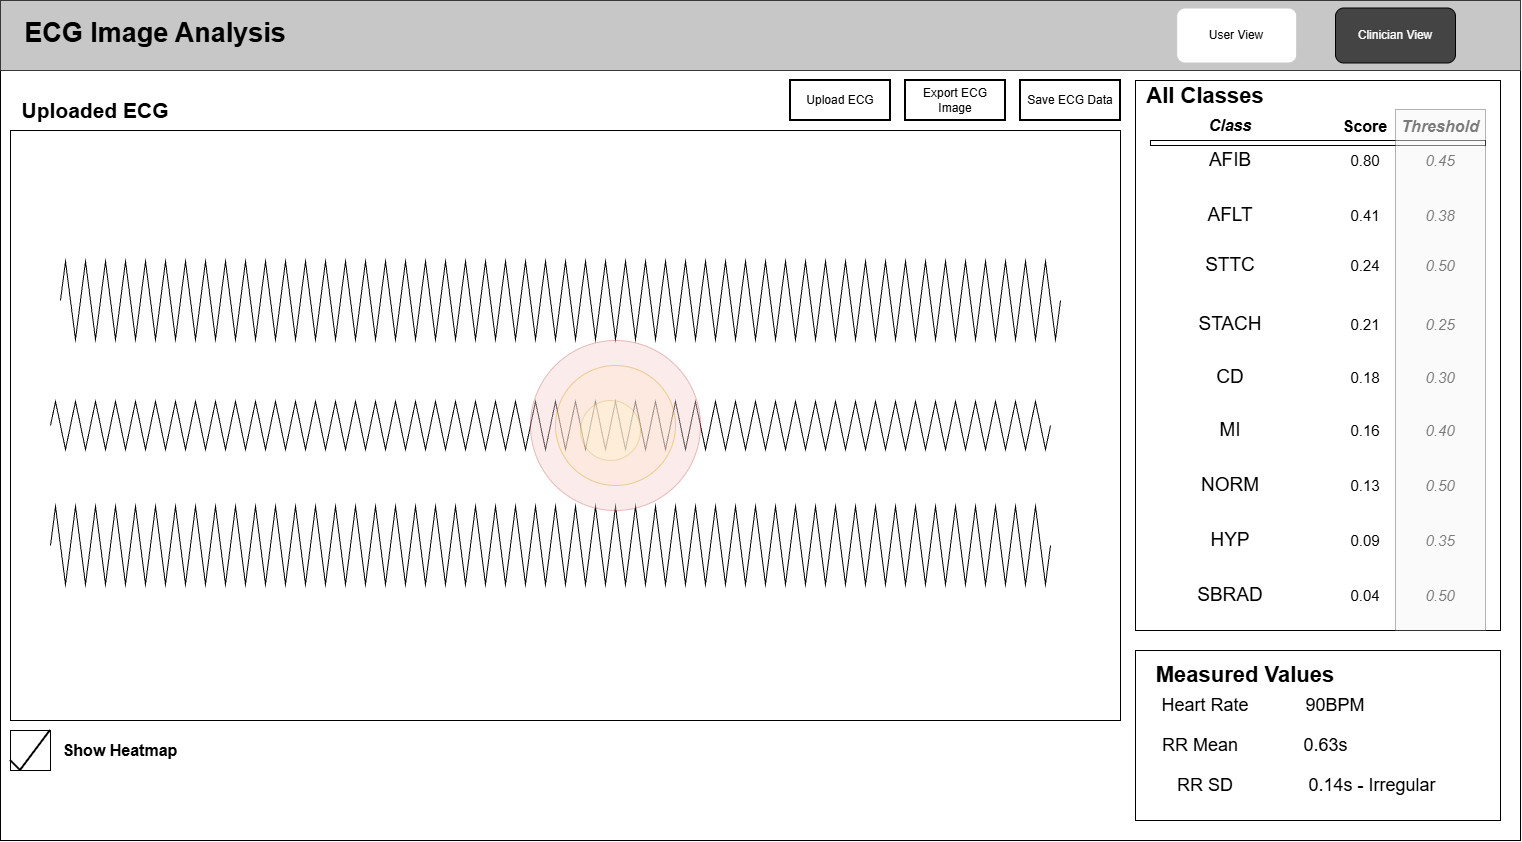
\includegraphics[width=0.85\linewidth,height=0.5\textheight,keepaspectratio]{images/clinician_view.png}
  \caption{Prototype 3: Wireframe created of the clinician view.}
  \label{fig:proto3clin}
\end{figure}


\chapter{Requirements Traceability Matrix}
\label{app:rtm}

Tables~\ref{tab:rtm-fr} and~\ref{tab:rtm-nfr} map each requirement in Table~\ref{tab:functional-req} to the module that implements it, its deliverable and its test case. The result column will be completed after system testing. The Won't requirements (FR16 and FR17) are not implemented, so they are not tested.

\begin{table}[H]
  \centering
  \footnotesize
  \setlength{\arrayrulewidth}{0.8pt}
  \renewcommand{\arraystretch}{1.25}
  \caption{Requirements Traceability Matrix: functional requirements.}
  \label{tab:rtm-fr}
  \begin{tabular}{|p{0.07\linewidth}|p{0.15\linewidth}|p{0.16\linewidth}|p{0.39\linewidth}|p{0.08\linewidth}|}
    \hline
    \rowcolor{cyan!90!black}
    \textcolor{white}{\textbf{ID}} & \textcolor{white}{\textbf{Module}} &
    \textcolor{white}{\textbf{Deliverable}} & \textcolor{white}{\textbf{Test case}} &
    \textcolor{white}{\textbf{Result}} \\
    \hline
    FR01 & GUI & Upload screen & TC01: Upload a scan and a photograph (PNG and JPG); both load and are displayed. & \\
    \hline
    FR02 & Preprocessing & Preprocessing module & TC02: Run on 20 rendered and 20 real images; the output keeps the trace, removes the grid and records the grid scale. & \\
    \hline
    FR03 & Detection & R-peak detector & TC03: On images with a source signal, at least 90\% of R peaks are found within $\pm150$\,ms of Pan--Tompkins. & \\
    \hline
    FR04 & Detection & Timing features & TC04: Heart-rate mean absolute error is at most 5\,bpm against the source signal. & \\
    \hline
    FR05 & Classifier & Trained CNN & TC05: A score is produced for each of the five superclasses on the test fold (performance tested by TC17). & \\
    \hline
    FR06 & Classifier & Trained CNN & TC06: A score is produced for each rhythm class; performance is reported where class counts allow. & \\
    \hline
    FR07 & Calibration, GUI & Results screen & TC07: Each flag shows a probability between 0 and 1, taken after temperature scaling. & \\
    \hline
    FR08 & Explanation, GUI & Heatmap overlay & TC08: A heatmap aligned with the image is shown for each flagged class. & \\
    \hline
    FR09 & GUI & Results screen & TC09: The HR and RR values shown match the detector output. & \\
    \hline
    FR10 & GUI & Explanation text & TC10: Each of the nine classes shows its plain-language description when flagged. & \\
    \hline
    FR11 & GUI & Wave diagram & TC11: The labelled diagram opens from the results screen. & \\
    \hline
    FR12 & GUI & Clinical view & TC12: Switching view shows only the flag list and measured values. & \\
    \hline
    FR13 & GUI & Export function & TC13: The exported file opens and contains the flags and scores. & \\
    \hline
    FR14 & GUI & Save function & TC14: A saved result reloads with the same contents. & \\
    \hline
    FR15 & Preprocessing, Detection & Quality check & TC15: On 20 heavily degraded images a warning is shown and no flags are given; on 20 clean images no warning is shown. & \\
    \hline
  \end{tabular}
\end{table}

\begin{table}[H]
  \centering
  \footnotesize
  \setlength{\arrayrulewidth}{0.8pt}
  \renewcommand{\arraystretch}{1.25}
  \caption{Requirements Traceability Matrix: non-functional requirements.}
  \label{tab:rtm-nfr}
  \begin{tabular}{|p{0.07\linewidth}|p{0.15\linewidth}|p{0.16\linewidth}|p{0.39\linewidth}|p{0.08\linewidth}|}
    \hline
    \rowcolor{cyan!90!black}
    \textcolor{white}{\textbf{ID}} & \textcolor{white}{\textbf{Module}} &
    \textcolor{white}{\textbf{Deliverable}} & \textcolor{white}{\textbf{Test case}} &
    \textcolor{white}{\textbf{Result}} \\
    \hline
    NFR01 & Whole system & Integrated application & TC16: The time from upload to results is under 10\,s for each of 20 images on the development PC. & \\
    \hline
    NFR02 & Classifier & Evaluation report & TC17: Mean AUROC on PTB-XL fold 10 is at least 0.85 across the five superclasses. & \\
    \hline
    NFR03 & Calibration & Reliability diagrams & TC18: ECE is at most 0.05 for each reported class after scaling, and lower than before. & \\
    \hline
    NFR04 & Classifier & Rendered-to-real report & TC19: The fall in AUROC per class is at most 0.10 for the five superclasses. & \\
    \hline
    NFR05 & GUI & User-study results & TC20: At least 70\% of participants interpret the confidence and heatmap correctly; mean SUS is at least 68. & \\
    \hline
    NFR06 & GUI & Limitations panel & TC21: The results screen lists the classes with few or no real test images. & \\
    \hline
    NFR07 & GUI & Session handling & TC22: After the session closes, no uploaded image remains on disk. & \\
    \hline
    NFR08 & Repository & Scripts and environment file & TC23: Re-running the evaluation script from a fresh clone reproduces the reported metrics. & \\
    \hline
    NFR09 & Whole system & Integrated application & TC24: Inference runs on a laptop without a GPU. & \\
    \hline
    NFR10 & Architecture & Module interfaces & TC25: The own CNN is replaced with the pretrained model without changing the pipeline or GUI code. & \\
    \hline
  \end{tabular}
\end{table}

\chapter{Supplementary Literature Material}
\label{app:lit}

\begin{table}[H]
  \centering
  \footnotesize
  \caption{Key studies in deep learning for ECG classification.}
  \label{tab:ecg-studies}
  \begin{tabular}{@{}p{0.13\linewidth} p{0.27\linewidth} p{0.25\linewidth} p{0.25\linewidth}@{}}
    \toprule
    \textbf{Study} & \textbf{Input and data} & \textbf{Reported result} &
      \textbf{Limitation for this project} \\
    \midrule
    \textcite{hannun_cardiologist_2019} &
      Single-lead signals; 91,232 ECGs, 53,549 patients &
      12 rhythm classes; F1 0.837 vs.\ 0.780 for cardiologists &
      Single lead; signals, not images \\
    \textcite{ribeiro_automatic_2020} &
      12-lead signals; over two million exams &
      Six abnormalities; F1 above 80\%, specificity above 99\% &
      Signals, not images \\
    \textcite{strodthoff_deep_2021} &
      12-lead signals, PTB-XL &
      Convolutional models performed best &
      Signals; hidden weakness in subclasses \\
    \textcite{sangha_automated_2022} &
      Images generated from signals; printed ECGs to test &
      Strong performance on held-out, external and printed ECGs (0.98 AUROC average) &
      Training images are generated from signals \\
    \textcite{gliner_domain_2023} &
      79,226 scanned labelled ECGs plus unlabelled phone-captured frames &
      Average AUROC of 0.91 on phone-captured images &
      Phone images made by filming printed pages; six unseen formats tested \\
    \textcite{wang_pipeline_2025} &
      Synthetic PTB-XL images plus external scanned sets &
      AUROC about 0.97 on the hidden test set &
      Synthetic test data; possible leakage from PTB-XL \\
    \bottomrule
  \end{tabular}
\end{table}

\begin{figure}[H]
  \centering
  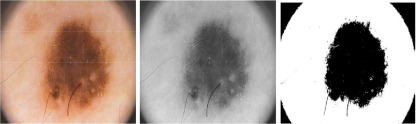
\includegraphics[width=0.38\linewidth]{images/OtsuSegmentation.jpg}
  \caption[Otsu segmentation of a dermatoscopic image]{Example of Otsu thresholding (Table~\ref{tab:techniques}) on a dermatoscopic image from the \(PH^2\) dataset. Reproduced from \cite{mendonca_ph_2013}.}
  \label{fig:otsu-dermatoscopic}
\end{figure}

\begin{figure}[H]
  \centering
  \begin{subfigure}[b]{0.35\linewidth}
    \centering
    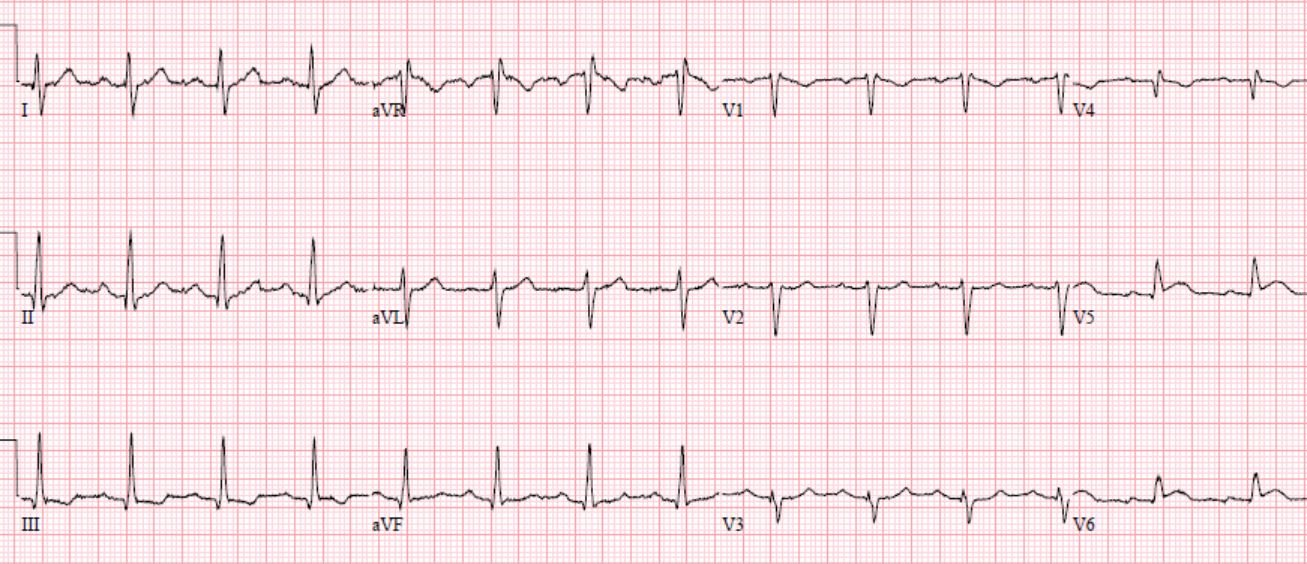
\includegraphics[width=\linewidth]{images/ecg_norm.jpg}
    \caption{Standard ECG Image.}
    \label{fig:ecgnorm}
  \end{subfigure}\hfill
  \begin{subfigure}[b]{0.35\linewidth}
    \centering
    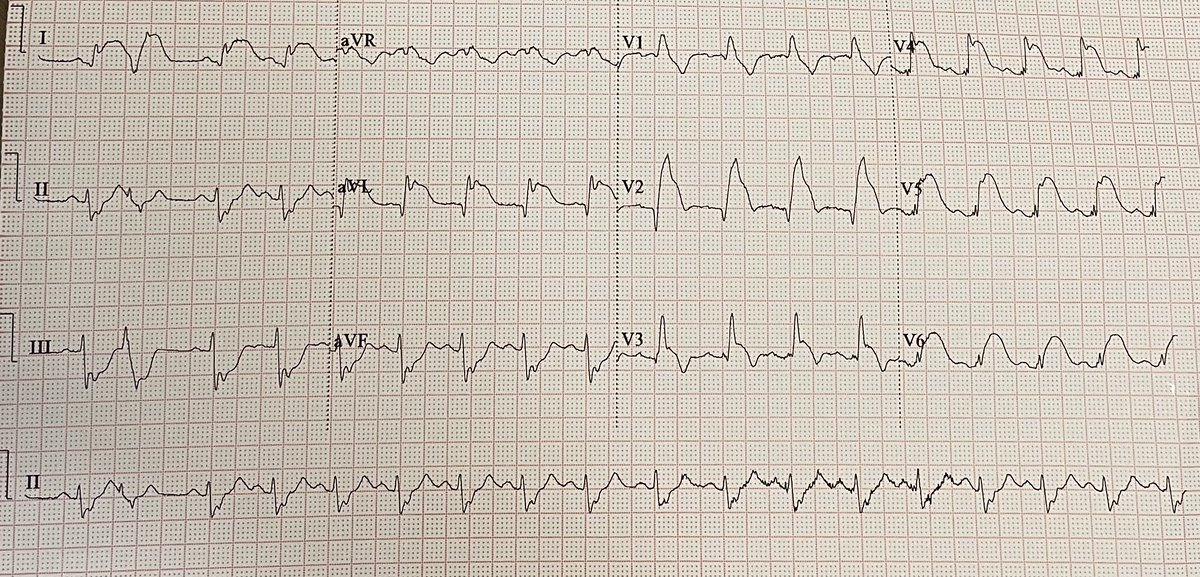
\includegraphics[width=\linewidth]{images/ecg_pict.jpg}
    \caption{ECG photographed (grid distorted).}
    \label{fig:ecgpict}
  \end{subfigure}\hfill
  \begin{subfigure}[b]{0.35\linewidth}
    \centering
    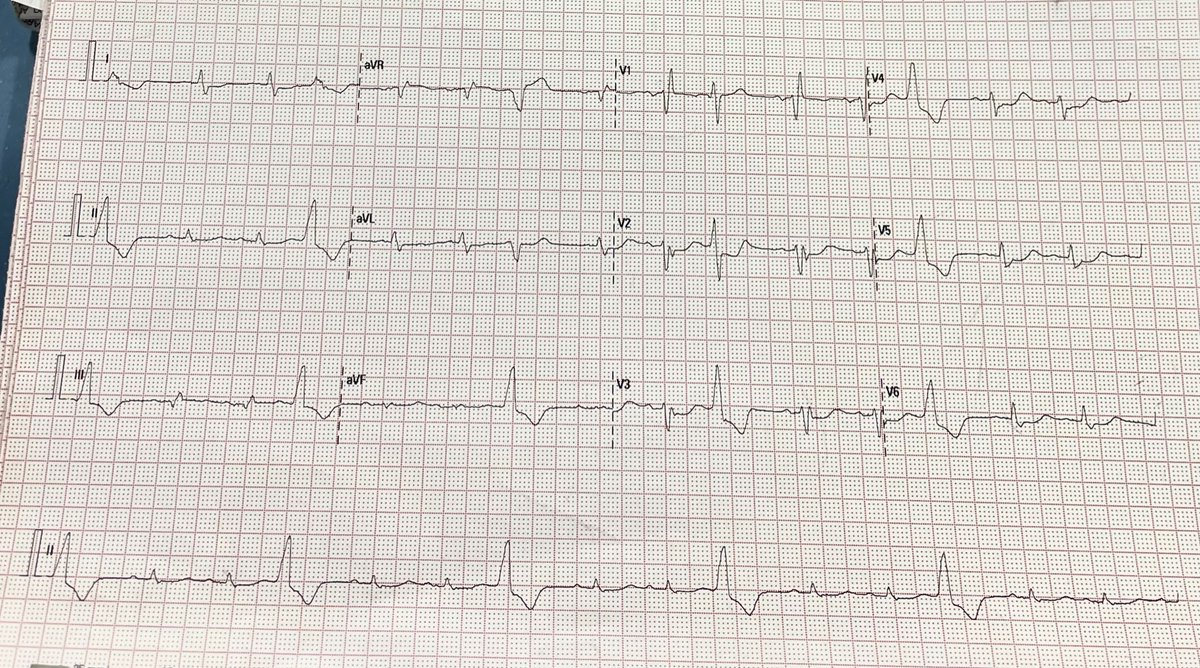
\includegraphics[width=\linewidth]{images/ecg_rotat.jpg}
    \caption{ECG photographed, with rotation.}
    \label{fig:ecgrotat}
  \end{subfigure}\hfill
  \begin{subfigure}[b]{0.35\linewidth}
    \centering
    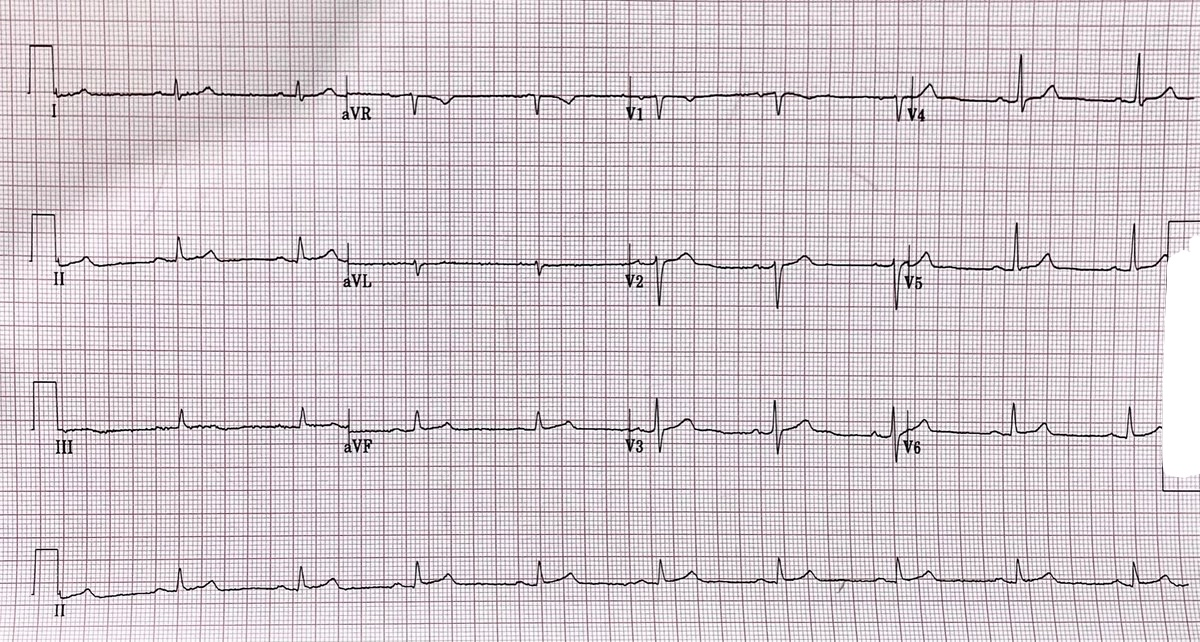
\includegraphics[width=\linewidth]{images/ecg_crease.jpg}
    \caption{ECG with a crease.}
    \label{fig:ecgcrease}
  \end{subfigure}\hfill
  \begin{subfigure}[b]{0.35\linewidth}
    \centering
    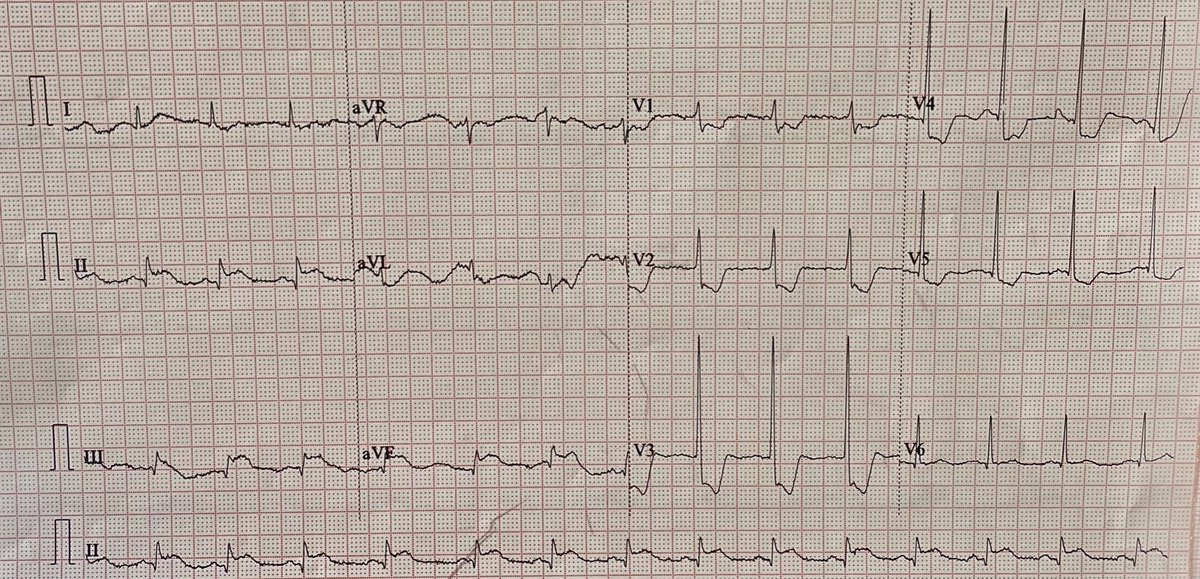
\includegraphics[width=\linewidth]{images/ecg_mark.jpg}
    \caption{ECG with pencil marks on them.}
    \label{fig:ecgmark}
  \end{subfigure}
  \caption{Various types of ECG images from the ECG-Image-Database.}
  \label{fig:ecgimages}
\end{figure}
\chapter*{Glossary}
\addcontentsline{toc}{chapter}{Glossary}
\label{glossary}

\begingroup
\small
\renewcommand{\arraystretch}{1.5}
\begin{longtable}{@{}>{\raggedright\arraybackslash}p{0.27\linewidth} p{0.68\linewidth}@{}}
  \toprule
  \textbf{Term} & \textbf{Definition} \\
  \midrule
  \endfirsthead
  \toprule
  \textbf{Term} & \textbf{Definition} \\
  \midrule
  \endhead
  \bottomrule
  \endfoot
  \textbf{Arrhythmia} & Any abnormal heart rate or rhythm. \\
  \textbf{Atrial fibrillation (AFIB)} & An arrhythmia in which the atria beat irregularly, giving irregularly spaced beats without clear P waves. \\
  \textbf{Atrial flutter (AFLT)} & An arrhythmia with a rapid, regular atrial rhythm that appears as a saw-tooth pattern. \\
  \textbf{AUROC} & Area under the receiver operating characteristic curve: the probability that a classifier scores a random positive case above a random negative one. 0.5 is chance and 1.0 is perfect; it does not depend on a threshold. \\
  \textbf{Augmentation} & Artificially altering training images (for example adding blur, shadows or rotation) so the model learns to cope with real-world variation. \\
  \textbf{Bootstrap confidence interval} & A range for a metric found by repeatedly resampling the test set with replacement; used when classes are small. \\
  \textbf{Bundle branch block (BBB)} & A conduction disturbance in which one of the heart's bundle branches is blocked, widening the QRS complex. \\
  \textbf{Calibration} & How well a model's stated confidence matches how often it is correct; a calibrated 80\% prediction is right about 80\% of the time. \\
  \textbf{CLAHE} & Contrast-limited adaptive histogram equalisation: histogram equalisation applied to small regions, with a limit on contrast to avoid amplifying noise. \\
  \textbf{CNN} & Convolutional neural network: a neural network that learns small image filters, stacking layers to build up from edges to complex patterns. \\
  \textbf{Conduction disturbance (CD)} & An abnormality in how the electrical impulse travels through the heart, such as a bundle branch block. \\
  \textbf{Data leakage} & When information from the test set is present in training, making results look better than they would be on unseen data. \\
  \textbf{Domain adaptation} & Techniques that adapt a model trained on one kind of data (for example scans) to another (for example phone photographs). \\
  \textbf{ECE} & Expected calibration error: the weighted average gap between predicted confidence and observed frequency, over confidence bins. Lower is better. \\
  \textbf{ECG} & Electrocardiogram: a recording of the heart's electrical activity, taken from electrodes on the body surface. \\
  \textbf{ECG-Image-Database} & A public dataset of about 36,000 real images of printed ECGs (from PTB-XL and Emory Healthcare) that were degraded and then scanned or photographed. \\
  \textbf{ECG-Image-Kit} & A software tool that renders ECG signals into synthetic ECG images, optionally with artefacts. \\
  \textbf{Fold} & One of the fixed subsets a dataset is divided into; PTB-XL provides ten patient-wise folds for training, validation and testing. \\
  \textbf{FR / NFR} & Functional requirement (what the system does) / non-functional requirement (how well it does it). \\
  \textbf{Grad-CAM} & Gradient-weighted class activation mapping: a method that produces a heatmap of the image regions that most influenced a CNN's prediction for a class. \\
  \textbf{GUI} & Graphical user interface. \\
  \textbf{Heart rate (HR)} & Beats per minute, calculated from the RR interval as $60/\mathrm{RR}$. \\
  \textbf{Histogram equalisation (HE)} & Spreading an image's intensity values across the full range to increase contrast. \\
  \textbf{Hough transform} & A technique for detecting straight lines (such as grid lines or lead baselines) in an image. \\
  \textbf{Hypertrophy (HYP)} & Thickening of a heart chamber's wall, associated with changes in ECG amplitude. \\
  \textbf{Lead} & One of the twelve views of the heart's electrical activity recorded in a standard ECG. \\
  \textbf{MCC} & Matthews correlation coefficient: a single measure of classification quality, from $-1$ to $1$, that remains informative when classes are imbalanced. \\
  \textbf{MI} & Myocardial infarction (heart attack): damage to heart muscle from a loss of blood supply, often visible as ST-segment and T-wave changes. \\
  \textbf{MoSCoW} & A prioritisation method that rates requirements as Must, Should, Could or Won't have. \\
  \textbf{Multi-label classification} & Classification in which one input can belong to several classes at once, each with its own output. \\
  \textbf{Otsu thresholding} & A method that automatically chooses the intensity cut-off separating foreground from background. \\
  \textbf{P wave, QRS complex, T wave }& The deflections of one heartbeat: atrial activation, ventricular activation and ventricular recovery. \\
  \textbf{Pan--Tompkins algorithm} & A standard real-time algorithm for detecting QRS complexes in an ECG signal. \\
  \textbf{PLES} & Professional, legal, ethical and social issues. \\
  \textbf{PTB-XL} & A public dataset of 21,800 labelled twelve-lead ECG signals from about 19,000 patients. \\
  \textbf{RR interval} & The time between successive R peaks, used to measure heart rate and rhythm regularity. \\
  \textbf{RTM} & Requirements Traceability Matrix: a table mapping each requirement to its design element, deliverable, test case and result. \\
  \textbf{Sensitivity} & The share of true cases a classifier finds: $\mathrm{TP}/(\mathrm{TP}+\mathrm{FN})$. \\
  \textbf{Shortcut learning} & When a model relies on features that happen to correlate with the label in training data (such as printed text) instead of the features that matter. \\
  \textbf{Sinus bradycardia / tachycardia} & A normal rhythm that is slower than 60 / faster than 100 beats per minute. \\
  \textbf{SNR} & Signal-to-noise ratio: the strength of a signal relative to background noise, usually in decibels. \\
  \textbf{Specificity} & The share of non-cases a classifier correctly clears: $\mathrm{TN}/(\mathrm{TN}+\mathrm{FP})$. \\
  \textbf{ST/T change (STTC)} & Changes to the ST segment or T wave, often linked to ischaemia. \\
  \textbf{SUS} & System Usability Scale: a standard ten-item questionnaire giving a usability score from 0 to 100, where 68 is average. \\
  \textbf{Temperature scaling} & A calibration method that divides each class score by a single value $T$, fitted on validation data, before the sigmoid. \\
  \textbf{Transfer learning} & Starting from a network pretrained on another task (for example natural images) and fine-tuning it for the new task. \\
\end{longtable}
\endgroup
	\backmatter
	\printbibliography[heading=bibintoc,title={References}]

    \printindex

    \end{document}
	







